\documentclass[a4paper,12pt]{article}

\usepackage{graphicx}
\usepackage{framed}
\usepackage{float}
\usepackage{amsmath}
\usepackage{booktabs}
\usepackage{titlesec}
\usepackage{tocloft}
\usepackage{geometry}
\usepackage{hyperref}

% Reduce margins
\geometry{
  a4paper,
  left=20mm,
  right=20mm,
  top=20mm,
  bottom=20mm,
}

% Reduce font size of section and subsection titles
\titleformat{\section}{\large\bfseries}{\thesection}{1em}{}
\titleformat{\subsection}{\normalsize\bfseries}{\thesubsection}{1em}{}

% Reduce spacing in Table of Contents
\setlength{\cftbeforesecskip}{5pt}
\setlength{\cftbeforesubsecskip}{2pt}

% Reduce space around floats (figures and tables)
\setlength{\textfloatsep}{10pt plus 1.0pt minus 2.0pt}
\setlength{\floatsep}{10pt plus 1.0pt minus 2.0pt}
\setlength{\intextsep}{10pt plus 1.0pt minus 2.0pt}

% Remove red bozes in table of contents
\hypersetup{pdfborder=0 0 0}

\title{E4D-HR User Guide}
\author{ExploreGeo}
\date{\today}

\begin{document}

\maketitle

\newpage

\tableofcontents

\newpage

\section{Introduction}

E4D-HR is a modified version of E4D, with changes made for mineral exploration use cases and some additional user-friendly features. E4D is a scalable, 3D geophysical modelling and inversion code designed to efficiently handle large datasets from direct current resistivity (DCR) and induced polarisation (IP) surveys.

This document is intended to guide geophysicists, who are familiar with DCR and IP methods, in using E4D to invert their data.


\section{Installation}

\subsection{System Requirements}

E4D-HR is compatible with the following Linux distributions. Windows users with versions that support WSL2 (Windows Subsystem for Linux) are also supported.

\begin{itemize}
    \item \textbf{Ubuntu:} 20.04 (Focal Fossa), 22.04 (Jammy Jellyfish), 24.04 (Noble Numbat)
    \item \textbf{WSL2:} Windows 10 (Version 1903 or later), Windows 11
\end{itemize}

\subsection{Required Software}

\begin{itemize}
    \item \textbf{Intel oneAPI Base Toolkit} 2024.2.0 or later
    \item \textbf{Intel HPC Toolkit} 2024.2.0 or later
    \item \textbf{build-essential} (Ubuntu and Debian)
    \begin{itemize}
        \item Install by running: \texttt{sudo apt-get update \&\& sudo apt-get install build-essential}
    \end{itemize}
\end{itemize}

\subsection{Downloading E4D}

To download E4D-HR, follow these steps:

\begin{enumerate}
    \item Visit the \href{https://github.com/ofgn/E4D-HR}{E4D-HR GitHub repository}.
    \item On the repository page, click on the \textbf{Code} button.
    \item You can either:
    \begin{itemize}
        \item \textbf{Clone the repository} using Git by running the following command in your terminal:
        \begin{verbatim}
git clone https://github.com/ofgn/E4D-HR.git
        \end{verbatim}
        \item \textbf{Download the ZIP file} by clicking on \textbf{Download ZIP}, and then extract the contents to your desired directory.
    \end{itemize}
\end{enumerate}

\subsection{Automatic Installation}

For an automatic installation of E4D, use the provided \texttt{install.sh} script. This script handles the downloading, extracting, compiling, and setting up of all dependencies and E4D itself. To use the script, follow these steps:

\begin{enumerate}
    \item Ensure that the necessary environment variables for Intel MKL are set.
    \item Open a terminal and navigate to the directory where \texttt{install.sh} is located.
    \item Make the script executable: \begin{verbatim}
chmod +x install.sh \end{verbatim}
    \item Run the script:  \begin{verbatim}
./install.sh   \end{verbatim}
    \item The script will automatically handle the installation of dependencies and E4D compilation. Follow any prompts provided by the script.
\end{enumerate}

Using the automatic installation script simplifies the setup process and ensures that all components are installed correctly with minimal manual intervention.

\subsection{Manual Installation}

To manually install E4D, follow these steps:

\begin{enumerate}
    \item \textbf{Prepare Your Environment}:
        \begin{itemize}
            \item Ensure that the Intel MKL environment variables are set. Source the Intel environment variables script (replace \texttt{<intel-compiler-dir>} with the path to your Intel installation):
            \begin{verbatim}
source <intel-compiler-dir>/setvars.sh
            \end{verbatim}
            \item Verify that the \texttt{MKLROOT} environment variable is set by running:
            \begin{verbatim}
echo $MKLROOT
            \end{verbatim}
            \item If \texttt{MKLROOT} is not set, refer to Intel’s documentation or support for configuration instructions.
        \end{itemize}

    \item \textbf{Install Dependencies}:
        \begin{itemize}
            \item \textbf{Install PETSc}:
                \begin{itemize}
                    \item Download and extract the PETSc source tarball (version 3.21.4):
                    \begin{verbatim}
tar -xzf petsc-3.21.4.tar.gz
                    \end{verbatim}
                    \item Navigate to the extracted directory:
                    \begin{verbatim}
cd petsc-3.21.4
                    \end{verbatim}
                    \item Configure PETSc with the appropriate options:
                    \begin{verbatim}
./configure --with-debugging=0 --with-fc=mpiifort -fc=ifx \\
--with-cc=mpiicc -cc=icx --with-cxx=mpiicpc -cxx=icpx \\
--with-blaslapack-dir=$MKLROOT
                    \end{verbatim}
                    \item Compile PETSc:
                    \begin{verbatim}
make all
                    \end{verbatim}
                \end{itemize}
            \item \textbf{Install Triangle}:
                \begin{itemize}
                    \item Download and extract the Triangle source tarball (version 1.6):
                    \begin{verbatim}
tar -xzf triangle-1.6.tar.gz
                    \end{verbatim}
                    \item Navigate to the extracted directory:
                    \begin{verbatim}
cd triangle-1.6
                    \end{verbatim}
                    \item Compile Triangle:
                    \begin{verbatim}
make
                    \end{verbatim}
                \end{itemize}
            \item \textbf{Install TetGen}:
                \begin{itemize}
                    \item Download and extract the TetGen source tarball (version 1.6.0):
                    \begin{verbatim}
tar -xzf tetgen-1.6.0.tar.gz
                    \end{verbatim}
                    \item Navigate to the extracted directory:
                    \begin{verbatim}
cd tetgen-1.6.0
                    \end{verbatim}
                    \item Compile TetGen:
                    \begin{verbatim}
make
                    \end{verbatim}
                \end{itemize}
        \end{itemize}

    \item \textbf{Compile E4D}:
        \begin{itemize}
            \item Navigate to the E4D source directory:
            \begin{verbatim}
cd path/to/E4D-HR/src
            \end{verbatim}
            \item Clean any previous builds:
            \begin{verbatim}
make clean
            \end{verbatim}
            \item Compile E4D with the configured PETSc:
            \begin{verbatim}
make FC=mpiifort -fc=ifx \\
FFLAGS="-O2 -xHost -r8 -heap-arrays" \\
PETSC_DIR=path/to/petsc-3.21.4
            \end{verbatim}
            \item Move the compiled E4D executable to the \texttt{bin} directory:
            \begin{verbatim}
mv e4d path/to/E4D-HR/bin
            \end{verbatim}
        \end{itemize}
\end{enumerate}


\newpage

\section{Background}

This section provides some technical details about E4D, which can be skipped. It offers context on the software’s capabilities and underlying principles, primarily for readers interested in the specific functionalities and computational methods employed in the modelling process.

\subsection{Complex Conductivity}

IP can be effectively described using the concept of complex conductivity, which captures both the conduction and polarisation properties of subsurface materials. E4D opts to use complex conductivity by decoupling the real and imaginary parts in the real number domain.

Complex conductivity \( \sigma^* \) is used to describe the electrical properties of subsurface regions. It is expressed as:

\begin{equation}
\sigma^* = \sigma' + i\sigma'',
\end{equation}

where \( \sigma' \) represents the conduction strength due to electromigration, and \( \sigma'' \) represents the polarisation strength associated with IP effects.

The phase \( \phi \) associated with \( \sigma^* \) is defined as:

\begin{equation}
\sigma^* = |\sigma^*| e^{i\phi},
\end{equation}

Here, \( \phi \) represents the phase lag of the induced alternating current (AC) electric field behind the injected AC current. The real part \( \sigma' \) is linked to the movement of charges through the material, while the imaginary part \( \sigma'' \) is associated with charge storage mechanisms, such as polarisation effects.

\subsubsection{Calculating Phase from Real and Imaginary Conductivity}

The phase \( \phi \) can be computed from the real part \( \sigma' \) and the imaginary part \( \sigma'' \) of the complex conductivity using the following equation:

\begin{equation}
\phi = \arctan\left(\frac{\sigma''}{\sigma'}\right),
\end{equation}

where \( \arctan \) denotes the inverse tangent function. This equation gives the phase in radians, representing the lag of the AC field relative to the current.

\subsubsection{Calculating Imaginary Conductivity from Real Conductivity and Phase}

The imaginary part of the complex conductivity \( \sigma'' \) can be calculated from the real part \( \sigma' \) and the phase \( \phi \) using:

\begin{equation}
\sigma'' = \sigma' \cdot \tan(\phi),
\end{equation}

where \( \tan \) denotes the tangent function. This formula derives the imaginary conductivity based on the known real conductivity and the phase angle.

\subsubsection{Magnitude of Complex Conductivity}

The magnitude of the complex conductivity \( |\sigma^*| \) is calculated as:

\begin{equation}
|\sigma^*| = \sqrt{(\sigma')^2 + (\sigma'')^2}.
\end{equation}


\subsection{Decoupling Real and Imaginary Components}

The use of complex numbers in E4D allows for the decoupling of the real and imaginary components of conductivity during forward and inverse modelling. This decoupling simplifies the computational process by allowing independent treatment of the real and imaginary components.

In typical IP surveys, the phase angle \( \phi \) is relatively small (e.g., less than 0.2 radians), which means the influence of the imaginary component on the real component is often negligible. This allows the real and imaginary parts to be modelled separately, reducing memory requirements by a factor of two and improving computational efficiency.

Moreover, this decoupling enables the specification of noise levels separately for the real and imaginary components of the potential (or equivalently, for the magnitude and phase), removing ambiguities in data misfit residuals that exist in the complex number domain. This approach ensures that the inversion process appropriately fits the data, leading to more accurate subsurface characterisation.



\subsection{DCR Data}

E4D expects the transfer resistance ($R_T$) as the DCR observation. $R_T$ is given in ohms and is the ratio of the primary voltage ($V_p$) and the applied current ($I$). Alternatively, it can be calculated as the ratio of the apparent resistivity ($\rho_a$) and the geometric factor ($K$) of the measurement's electrode configuration.

\begin{equation}
R_T = \frac{V_p}{I}
\end{equation}

\begin{equation}
R_T = \frac{\rho_a}{K}
\end{equation}

\subsection{IP Data}

E4D uses the phase difference in radians between the source and measured potentials for IP modelling. This approach differs from other inversion programs that may use integral chargeability, Cole-Cole parameters, or alternative methods. To accommodate data obtained through various techniques, a correction factor is applied for conversion purposes. While the specific value of the correction factor varies with different instruments and acquisition settings, Table 1 provides rough conversion factors for common IP measurements, which have generally yielded satisfactory results.

\begin{table}[H]
\centering
\begin{tabular}{@{}lc@{}}
\toprule
Unit                       & Conversion \\ \midrule
1 mrad                     & 0.001 rad         \\
1 mV/V                     & 0.001 rad         \\
1 ms                       & 0.001 rad         \\
1 Percent Frequency Effect & 0.01 rad          \\ \bottomrule
\end{tabular}
\caption{IP unit conversion.}
\end{table}

\subsection{Triangular Mesh}

A triangular mesh is a 2D mesh composed of interconnected triangles. In E4D, this type of mesh is primarily used to represent surfaces such as topography or other planar features. The triangles in the mesh are defined by vertices that correspond to control points, which could be surface electrodes or specific points on the topography. This triangular mesh serves as the foundation for more complex 3D meshes by accurately capturing the shape and variations of the surface it represents. The simplicity and flexibility of triangular meshes make them ideal for creating detailed surface representations that can be used as boundaries in 3D modelling processes.

\subsection{Tetrahedral Mesh}

E4D uses unstructured tetrahedral meshes for DCR and IP modelling. A tetrahedral mesh is a 3D mesh composed of tetrahedra, which are four-faced polyhedra where each face is a triangle. This structure allows the mesh to fill three-dimensional space effectively, making it suitable for modelling subsurface volumes.

Tetrahedral meshes offer significant geometric flexibility, allowing for the accurate representation of irregular surfaces and complex subsurface structures. This flexibility is crucial when incorporating complex topographies and heterogeneous subsurface conditions into the model. By using tetrahedra, the mesh can conform to the intricate details of the subsurface environment, ensuring that the simulations reflect real-world conditions as closely as possible.

Additionally, tetrahedral meshes enable targeted refinement around critical areas, such as around electrodes. This refinement improves numerical accuracy by increasing the mesh density where it is most needed, without significantly increasing the overall computational load. The result is a more efficient and accurate model, capable of handling the complexities of DCR and IP simulations.

\subsection{Constrained Tetrahedralisation}

In the process of generating a 3D mesh for subsurface modelling, accurately defining the upper surface is crucial. This surface is often irregular due to variations in topography or the placement of surface electrodes, which serve as control points in the mesh generation process.

To create this upper surface, E4D employs Triangle, a tool designed for generating high-quality triangulations. Triangle takes the control points, defined by the locations of surface electrodes or topographical data, and creates a triangulated surface. This triangulation ensures that the mesh closely conforms to the actual surface, capturing all significant features and variations. The resulting mesh is a collection of triangles, each defined by three vertices corresponding to the control points.

Once the upper surface has been triangulated, E4D uses this as a key component in constructing the 3D mesh. The vertical and lower surfaces, which are generally simpler and often defined as planes, are then joined with the upper surface. Together, these surfaces form the constraint for the tetrahedral mesh.

TetGen is then utilised to create the fully constrained tetrahedral mesh. It incorporates the triangulated upper surface from Triangle, along with the joined vertical and lower surfaces, as boundary conditions for the 3D mesh. This process, known as constrained tetrahedralisation, ensures that the triangles forming the upper surface are preserved as faces of the tetrahedra in the final mesh. This approach maintains the complexity and accuracy of the upper surface, leading to more reliable simulations of subsurface properties.


\subsection{Inversion}

Inversion can be understood as comprising two key components: forward modelling and the minimisation of an objective function. Forward modelling involves simulating how the earth's subsurface would respond to geophysical survey techniques, based on an initial set of model parameters. This simulated response is then compared to actual survey data, highlighting discrepancies between the model and reality. The process of minimisation of an objective function comes into play to adjust the model parameters iteratively, aiming to reduce the differences between the simulated and observed data. This minimisation effort seeks to find the set of model parameters that best fits the observed data, thereby enhancing the accuracy of the subsurface model. This iterative process continues until the model sufficiently conforms to the observed data, achieving a balance between fitting the data and maintaining a geologically plausible model structure.

\subsection{Forward Modelling}

E4D performs forward modelling by solving systems of equations for both real and imaginary components using the finite element method on an unstructured tetrahedral mesh, as detailed by \cite{johnson_3-d_2017} and \cite{rucker_three-dimensional_2006} respectively.

The unstructured design of the finite element mesh allows for the extension of mesh boundaries far from the source region, effectively mitigating boundary effects without significantly increasing the number of mesh elements.

E4D uses the third-party mesh generator TetGen \cite{10.1145/2629697} for mesh creation and a Krylov subspace solver from PETSc \cite{balay2019petsc} to solve the equations.

\begin{equation}
\mathbf{A}^\prime \boldsymbol {\phi}^\prime = I + \mathbf{A}^{\prime\prime}\boldsymbol {\phi}^{\prime\prime}
\end{equation}

\begin{equation}
\mathbf{A}^\prime \boldsymbol {\phi}^{\prime\prime} = -\mathbf{A}^{\prime\prime}\boldsymbol {\phi}^\prime
\end{equation}

$\mathbf{A}^\prime$ and $\mathbf{A}^{\prime\prime}$ are sparse $n \times n$ finite element coupling matrices, constructed using the real and imaginary components of conductivity respectively, including appropriate boundary conditions, where $n$ is the number of mesh nodes.

$\boldsymbol {\phi}^{\prime}$ and $\boldsymbol {\phi}^{\prime\prime}$ represent the $n$ element solution vectors holding the real and imaginary components of the potential field, respectively.

$I$ is an $n$ element vector holding the source current magnitude.

\subsection{Objective Function}

The goal of the inversion process is to refine the model by minimising an objective function that quantifies the discrepancy between the model's predictions and the observed data. The nonlinear conjugate gradient least squares (CGLS) algorithm is used to iteratively adjust the model to achieve this minimisation. 

Relying solely on the data misfit function, which measures the difference between the model's predictions and the collected data, would lead to an excessive number of free parameters. This could result in a wide range of potential models with varying degrees of geological realism. To address this, it is crucial to impose additional constraints on the model. A smoothness constraint is typically applied to guide the model towards a more geologically plausible configuration by penalising excessive variations.

The objective function can be divided into two main components:

\begin{equation}
\Phi (\mathbf{m}^{\text{est}}) = \Phi_d (\mathbf{m}^{\text{est}}) + \beta \Phi_m (\mathbf{m}^{\text{est}})
\end{equation}

$\Phi_d$ represents the data misfit. This term quantifies the difference between the observed data and the predicted data generated by the model.

\(\Phi_m\) represents the model norm, which imposes regularisation on the model parameters. This function is used to enforce desired structures in the recovered model, ensuring that the solution is both stable and geologically plausible. The value of \(\Phi_m\) is determined by applying structural metrics and weighting functions, which define the specific structures to be imposed and the conditions under which they influence the inversion process.

$\beta$ is a tunable coefficient that controls the weighting of the model constraints, most commonly the smoothness of the model. E4D has the option to start with a high $\beta$ to prioritise a smooth model and then gradually decrease $\beta$ to allow for increased model complexity as data fitting improves.

\(\mathbf{m}^{\text{est}}\) is a vector that consists of estimated conductivity values for each element in the computational mesh. The goal of the inversion is to find \(\mathbf{m}^{\text{est}}\) which accurately reflects the earth of the survey area.

\begin{framed}
\noindent \textbf{Important Note:} In the E4D log file, $\beta \Phi_m$ and $\Phi_m$ are reported as $\Phi_m$ and $\Phi_m / \beta$ respectively.
\end{framed}

\subsection{Structural Metrics} \label{structural_metrics}

A structural metric in E4D defines a relationship between the property (conductivity or phase) of a target element and one of the following:

\begin{itemize}
    \item The property of the target element's neighbouring elements.
    \item The specified reference property value (see \texttt{ref\_value} in the inverse options file syntax).
    \item The property of the corresponding element in the reference model file.
\end{itemize}

When a particular structural metric is assigned to a zone, E4D applies that metric to every element in that zone, and optionally to elements bounding that zone if specified in the corresponding constraint block. E4D then minimises the structural metric, thereby imposing the desired structure in the inverse solution.

The conditions under which E4D applies these constraints are determined by the weighting function associated with each structural metric. Therefore, the impact of each structural metric on constraining the inversion depends on the corresponding weighting function. The equations below describe each structural metric:

\begin{description}
    \item[\texttt{struct\_met = 1}:] The difference between the log of the property of the target element (\( m_t \)) and the log of the property of its neighbouring element (\( m_n \)). Mathematically, \( X = m_t - m_n \).
    
    \item[\texttt{struct\_met = 2}:] The absolute difference between the log of the property of the target element (\( m_t \)) and the log of the property of its neighbouring element (\( m_n \)). Mathematically, \( X = |m_t - m_n| \).
    
    \item[\texttt{struct\_met = 3}:] The difference between the log of the property of the target element (\( m_t \)) and the log of the reference property value (\texttt{v\_ref}). Mathematically, \( X = m_t - \texttt{v\_ref} \), where \texttt{v\_ref} is taken either from the constraint block or from the reference model file.
    
    \item[\texttt{struct\_met = 4}:] The absolute difference between the log of the property of the target element (\( m_t \)) and the log of the reference property value (\texttt{v\_ref}). Mathematically, \( X = |m_t - \texttt{v\_ref}| \).
    
    \item[\texttt{struct\_met = 5}:] Similar to \texttt{struct\_met = 1}, but with anisotropic weighting applied. Mathematically, \( X = m_t - m_n \), with anisotropic weighting in specific directions.
    
    \item[\texttt{struct\_met = 6}:] Similar to \texttt{struct\_met = 2}, but with anisotropic weighting applied. Mathematically, \( X = |m_t - m_n| \), with anisotropic weighting in specific directions.
    
    \item[\texttt{struct\_met = 7}:] Typically used for time-lapse inversion. It calculates the difference between the temporal change in the log of the property for spatially adjacent elements. Mathematically, \( X = (m_t - \texttt{v\_reft}) - (m_n - \texttt{v\_refn}) \), where \( m_t \) and \( m_n \) are the logs of the property of the target and neighbouring elements, respectively, and \( \texttt{v\_reft} \) and \( \texttt{v\_refn} \) are the reference values at a previous time.
    
    \item[\texttt{struct\_met = 8}:] Also used for time-lapse inversion, but it calculates the absolute difference between the temporal change in the log of the property for spatially adjacent elements. Mathematically, \( X = |(m_t - \texttt{v\_reft}) - (m_n - \texttt{v\_refn})| \).
    
    \item[\texttt{struct\_met = 9}:] Similar to \texttt{struct\_met = 1}, but applied only at specified boundaries. Mathematically, \( X = m_t - m_n \).
    
    \item[\texttt{struct\_met = 10}:] Similar to \texttt{struct\_met = 2}, but applied only at specified boundaries. Mathematically, \( X = |m_t - m_n| \).
\end{description}

\subsection{Weighting Functions} \label{weighting_functions}

The primary purpose of the weighting function is to determine the conditions under which the corresponding structural metric should or should not be used to constrain the inversion. In essence, the weighting functions activate or deactivate the structural metrics and determine the degree of emphasis on minimising the structural metric during the transition between activation and deactivation.

The independent variable for each weighting function is the value of the structural metric, denoted as \(X\). Each weighting function is based on the normal and cumulative normal distribution functions, and the output of these functions ranges between 0 and 1. If the weighting function evaluates to zero, the structural metric is inactive and does not influence the inversion. If it evaluates to one, the structural metric is fully active.

\begin{description}
    \item[Weighting Function 1:] Minimize \(X\) if \(X\) drops below \(\text{mn} + 2\text{sd}\), reaching full weight if \(X\) drops below \(\text{mn} - 2\text{sd}\).
    \begin{equation}
    f(X) = 0.5 \times \left(1 - \text{erf}\left(\frac{X - \text{mn}}{\sqrt{2} \times \text{sd}}\right)\right)
    \end{equation}
    \begin{figure}[H]
        \centering
        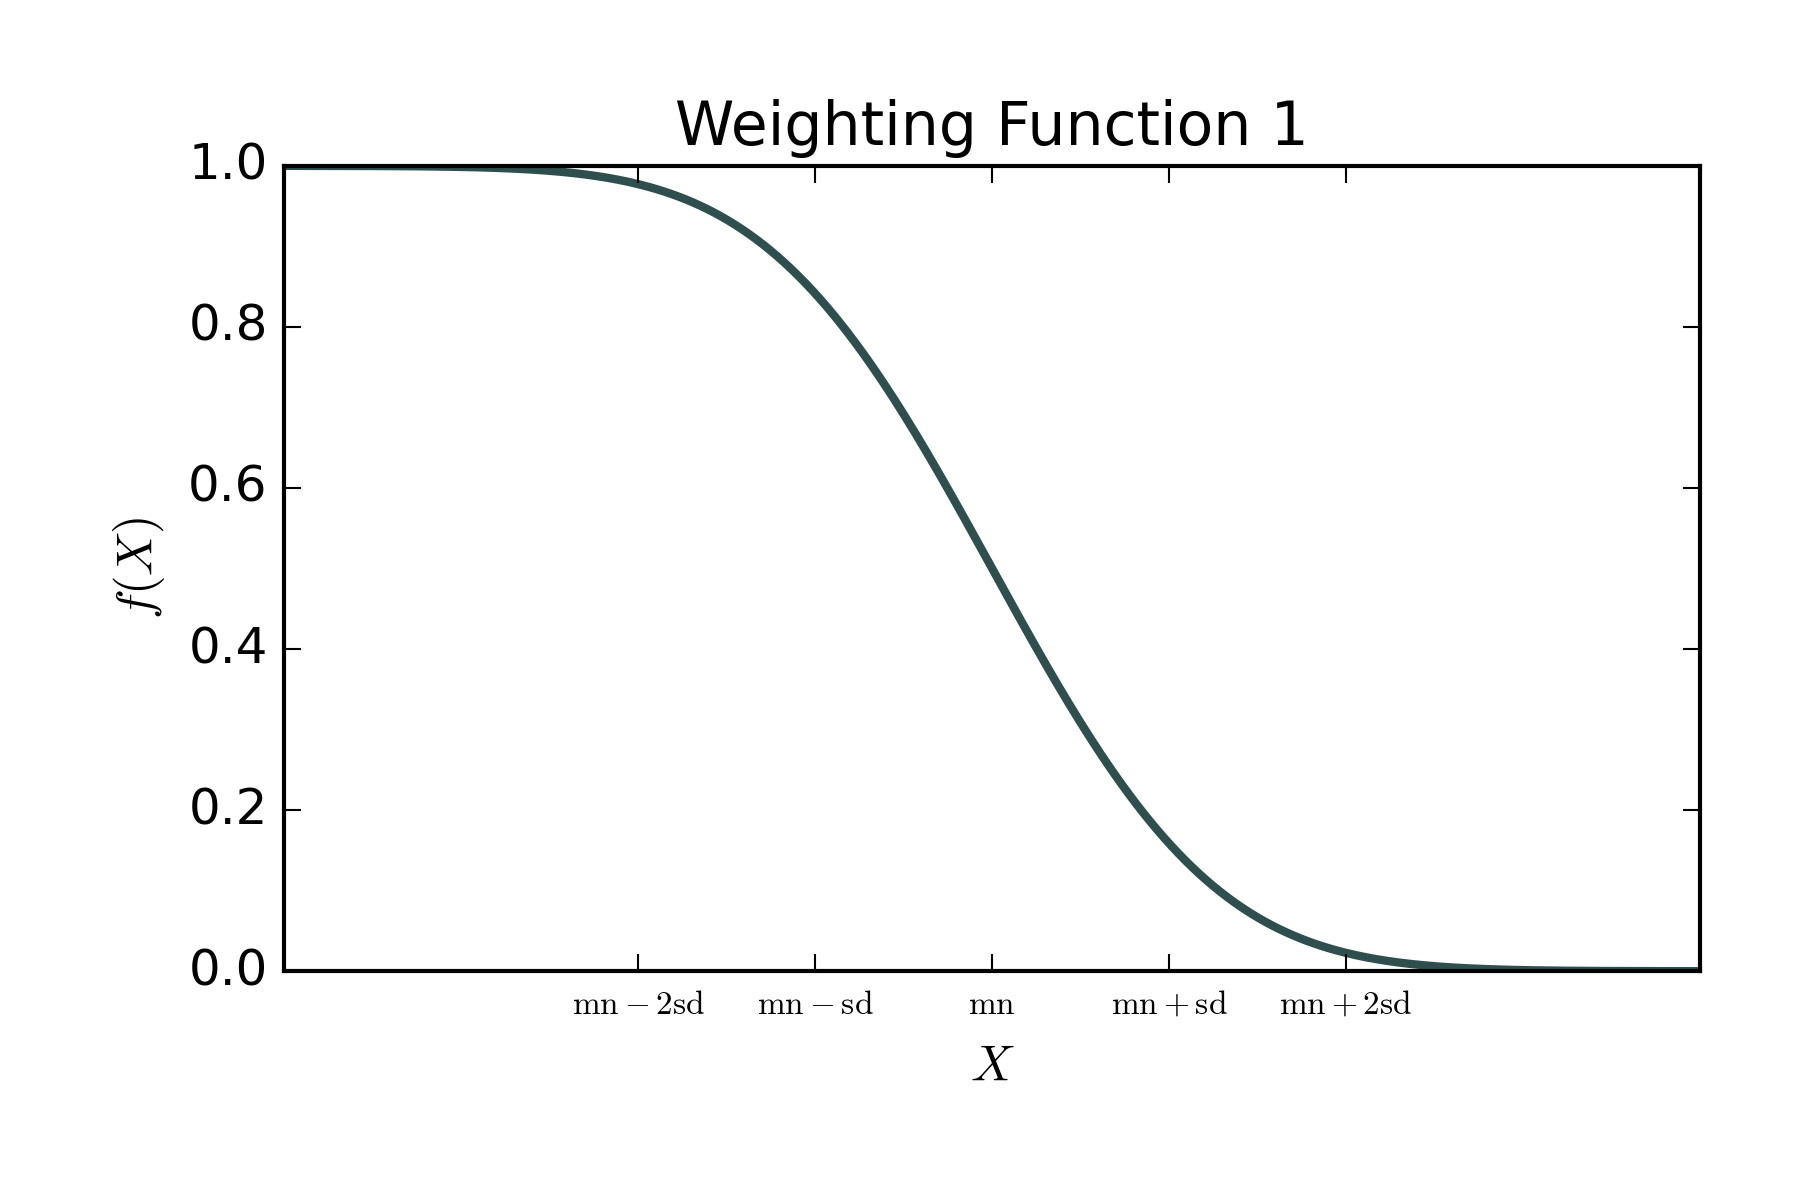
\includegraphics[width=0.8\textwidth]{figures/weighting_function_1.png}
        \caption{Weighting Function 1: \(f(X)\) decreases as \(X\) drops below \(\text{mn}\).}
    \end{figure}

    \item[Weighting Function 2:] Minimize \(X\) if \(X\) rises above \(\text{mn} - 2\text{sd}\), reaching full weight if \(X\) rises above \(\text{mn} + 2\text{sd}\).
    \begin{equation}
    f(X) = 0.5 \times \left(1 + \text{erf}\left(\frac{X - \text{mn}}{\sqrt{2} \times \text{sd}}\right)\right)
    \end{equation}
    \begin{figure}[H]
        \centering
        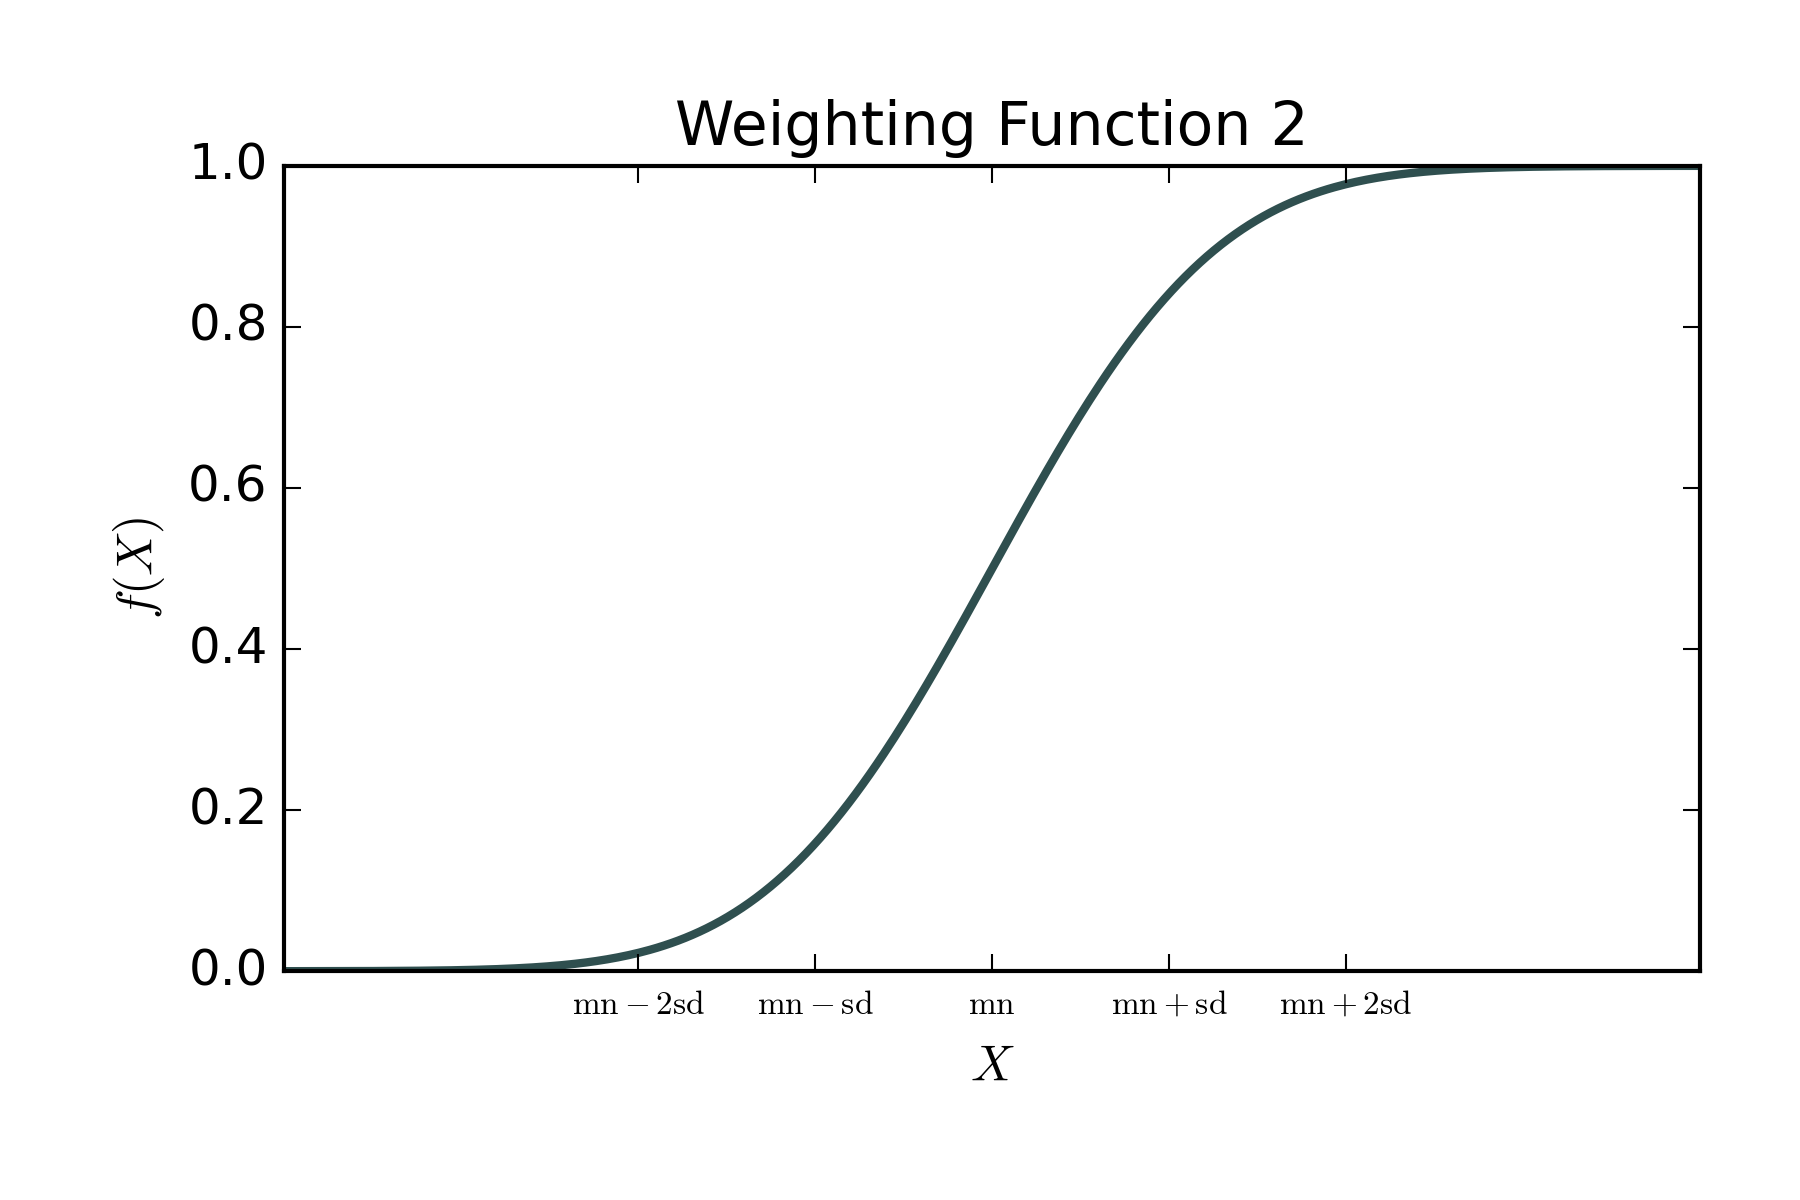
\includegraphics[width=0.8\textwidth]{figures/weighting_function_2.png}
        \caption{Weighting Function 2: \(f(X)\) increases as \(X\) rises above \(\text{mn}\).}
    \end{figure}

    \item[Weighting Function 3:] Minimize \(X\) if \(X\) deviates from \(\text{mn}\), reaching full weight if \(X\) deviates from \(\text{mn}\) by more than approximately \(2\text{sd}\).
    \begin{equation}
    f(X) = 1 - \exp\left(-\frac{(X - \text{mn})^2}{2 \times \text{sd}^2}\right)
    \end{equation}
    \begin{figure}[H]
        \centering
        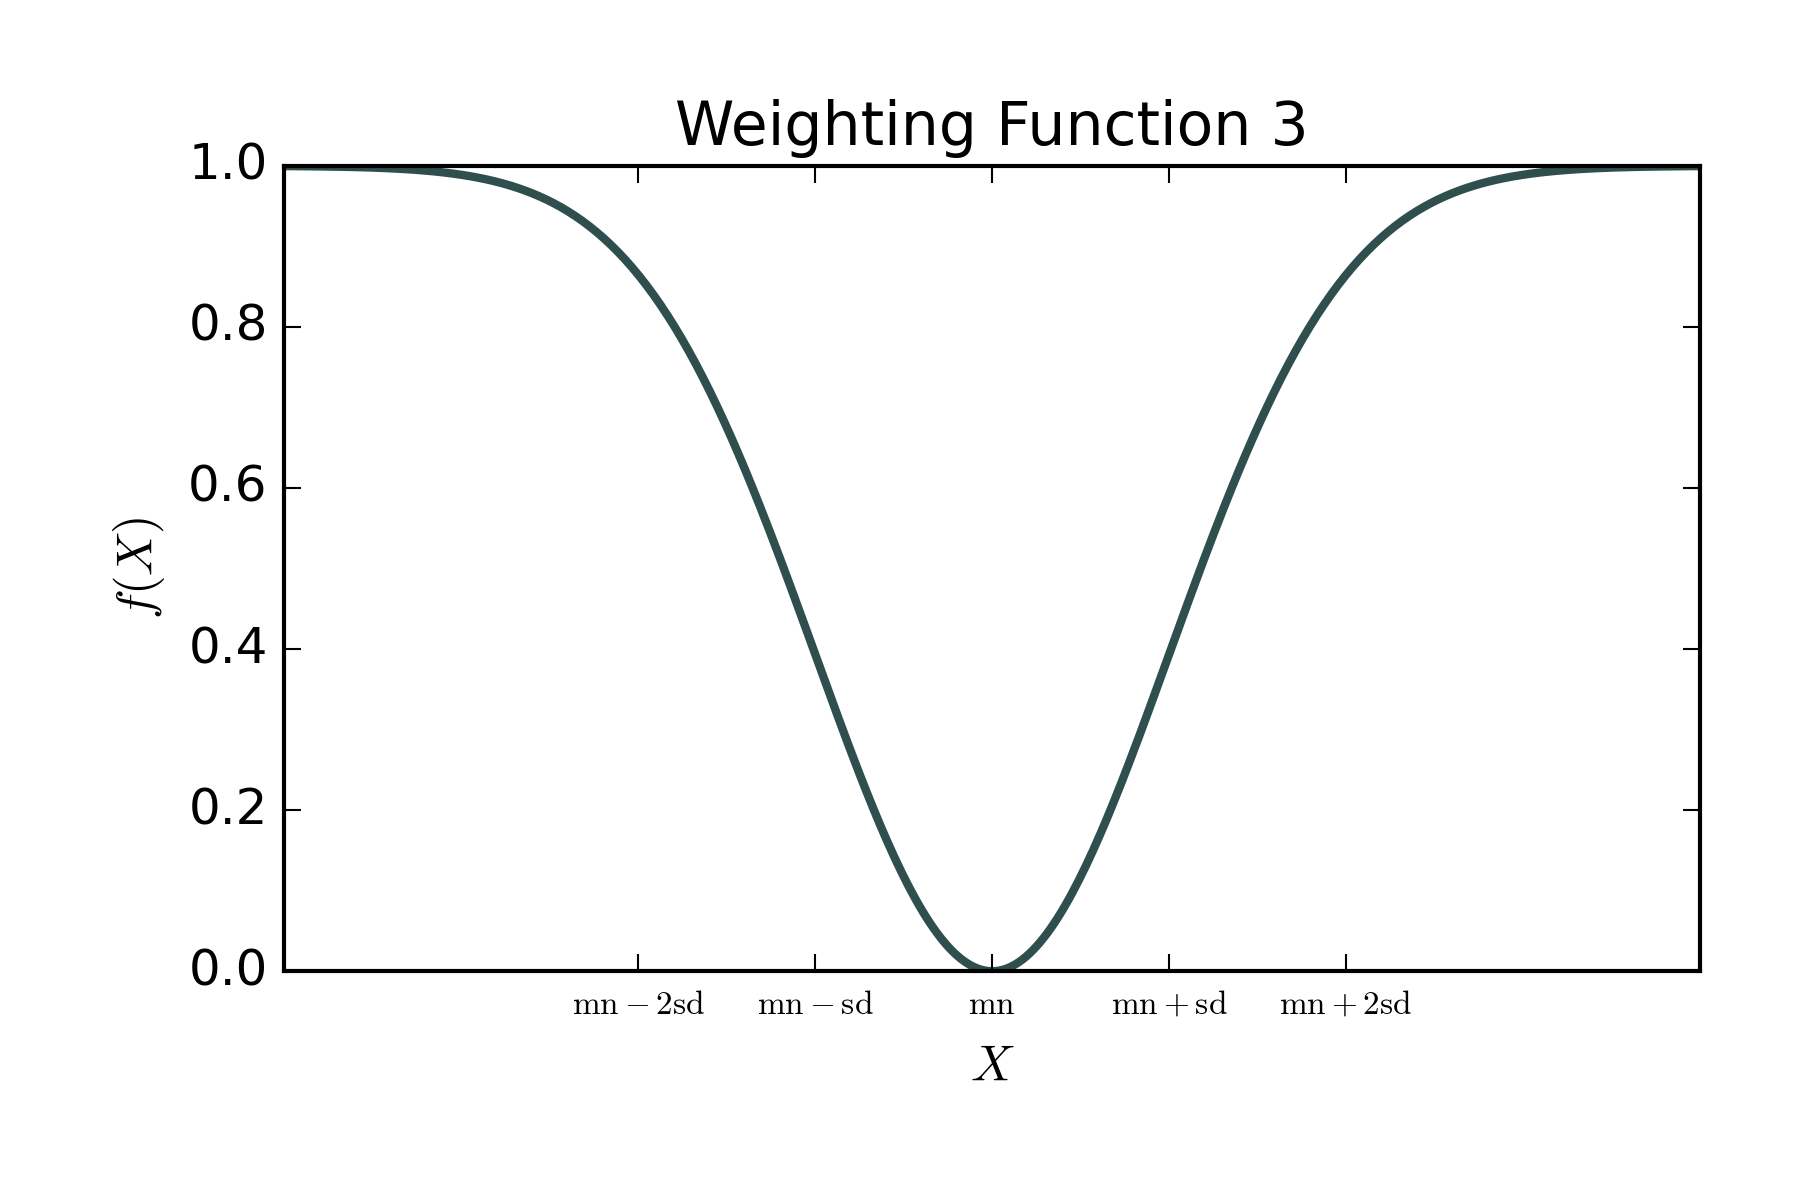
\includegraphics[width=0.8\textwidth]{figures/weighting_function_3.png}
        \caption{Weighting Function 3: \(f(X)\) increases as \(X\) deviates from \(\text{mn}\).}
    \end{figure}

    \item[Weighting Function 4:] Minimize \(X\) as \(X\) approaches \(\text{mn}\), reaching full weight when \(X\) equals \(\text{mn}\).
    \begin{equation}
    f(X) = \exp\left(-\frac{(X - \text{mn})^2}{2 \times \text{sd}^2}\right)
    \end{equation}
    \begin{figure}[H]
        \centering
        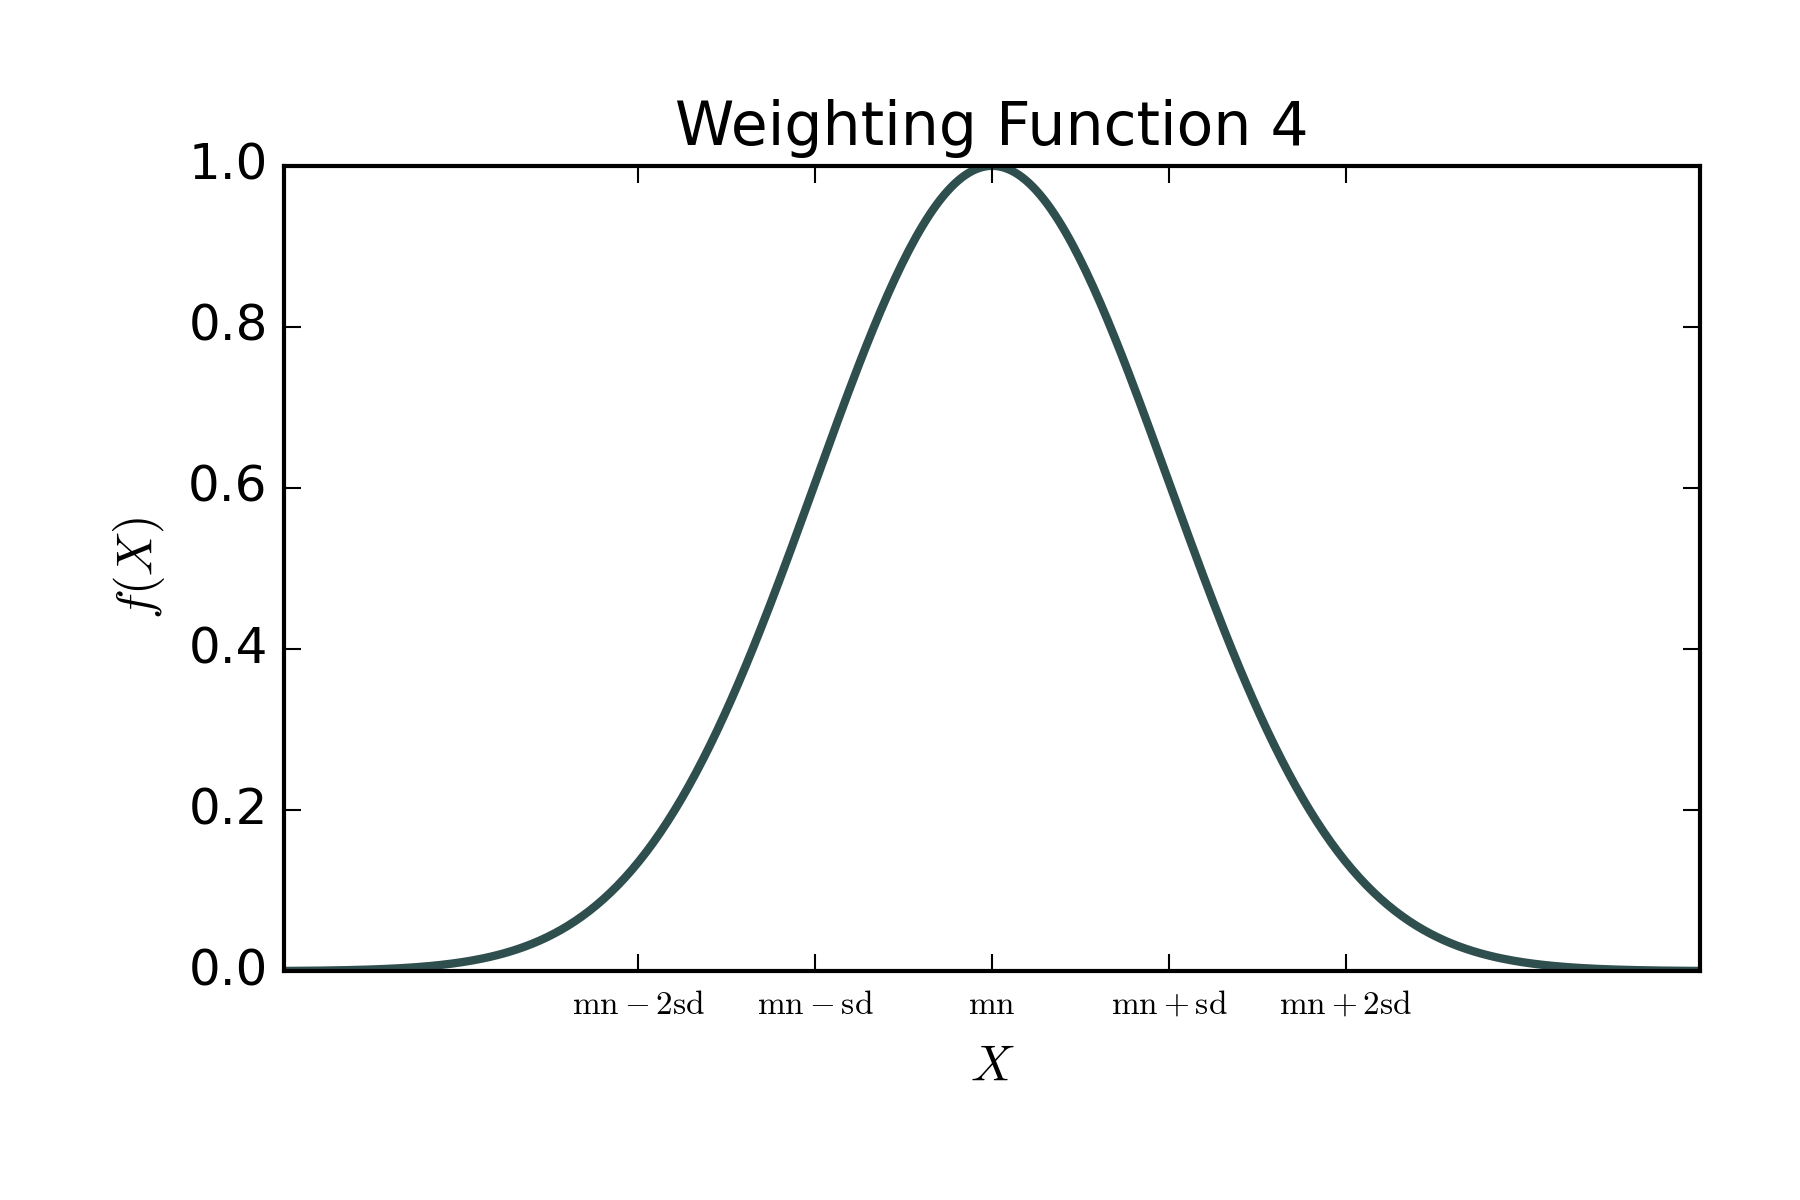
\includegraphics[width=0.8\textwidth]{figures/weighting_function_4.png}
        \caption{Weighting Function 4: \(f(X)\) decreases as \(X\) approaches \(\text{mn}\).}
    \end{figure}
\end{description}

The variables used in these equations are as follows:

\begin{itemize}
    \item \(f(X)\): The value of the weighting function, where \(0 \leq f(X) \leq 1\).
    \item \(X\): The value of the structural metric.
    \item \(\text{erf}\): The error function.
    \item \(\text{exp}\): The exponential function, where \(e = 2.718281828\).
    \item \(\text{mn}\): The mean of the weighting function, as specified in the constraint block in the inversion options file.
    \item \(\text{sd}\): The standard deviation of the weighting function, as specified in the constraint block in the inversion options file.
\end{itemize}

\section{Types of Constraints}

\subsection{Smoothness Constraint}
\begin{itemize}
    \item \textbf{Structural Metric}: Metric 2
    \begin{itemize}
        \item Encourages smooth variations between adjacent elements.
    \end{itemize}
    \item \textbf{Weighting Function}: Function 1
    \begin{itemize}
        \item \textbf{Mean}: Typically set to a high value (e.g., 10).
        \item \textbf{Standard Deviation}: Small (e.g., 0.01).
        \item Ensures that the smoothness constraint is applied only when the difference between adjacent elements is not extreme.
    \end{itemize}
\end{itemize}

\subsection{Minimum Conductivity Constraint}
\begin{itemize}
    \item \textbf{Structural Metric}: Metric 3
    \begin{itemize}
        \item Enforces a lower bound on conductivity values.
    \end{itemize}
    \item \textbf{Weighting Function}: Function 1
    \begin{itemize}
        \item \textbf{Mean}: Typically set to 0.
        \item \textbf{Standard Deviation}: Small (e.g., 0.1).
        \item \textbf{Reference Value}: Defines the minimum allowable conductivity (e.g., 0.002 S/m). When the log conductivity drops below this value, the constraint activates to ensure that conductivity does not fall below the specified minimum.
    \end{itemize}
\end{itemize}

\subsection{Maximum Conductivity Constraint}
\begin{itemize}
    \item \textbf{Structural Metric}: Metric 3
    \begin{itemize}
        \item Enforces an upper bound on conductivity values.
    \end{itemize}
    \item \textbf{Weighting Function}: Function 2
    \begin{itemize}
        \item \textbf{Mean}: Typically set to 0.
        \item \textbf{Standard Deviation}: Small (e.g., 0.1).
        \item \textbf{Reference Value}: Defines the maximum allowable conductivity (e.g., 0.01 S/m). When the log conductivity exceeds this value, the constraint activates to ensure that conductivity does not surpass the specified maximum.
    \end{itemize}
\end{itemize}

\subsection{Blocky Constraint}
\begin{itemize}
    \item \textbf{Structural Metric}: Metric 2
    \begin{itemize}
        \item Enforces blocky variations between adjacent elements.
    \end{itemize}
    \item \textbf{Weighting Function}: Function 1
    \begin{itemize}
        \item \textbf{Mean}: Lower than in smoothness constraints (e.g., 0.1).
        \item \textbf{Standard Deviation}: Small relative to the mean (e.g., 0.05).
        \item Enforces similarity constraints only if the difference between adjacent elements is relatively small, making the model more blocky rather than smooth.
    \end{itemize}
\end{itemize}

\subsection{Anisotropic Weighting and Inequality Constraints}
\begin{itemize}
    \item \textbf{Structural Metric}: Metric 6
    \begin{itemize}
        \item Encourages continuity normal to a specific plane.
    \end{itemize}
    \item \textbf{Weighting Function}: Function 1
    \begin{itemize}
        \item \textbf{Mean}: Set to a high value (e.g., 5.0).
        \item \textbf{Standard Deviation}: Small (e.g., 0.02).
        \item Applies constraints in an anisotropic manner based on the orientation of the plane.
    \end{itemize}
    \item \textbf{Inequality Constraints}:
    \begin{itemize}
        \item \textbf{Lower Bound}: Metric 3 with Weighting Function 1
        \begin{itemize}
            \item \textbf{Reference Value}: Defines the minimum bound (e.g., 0.001 S/m).
        \end{itemize}
        \item \textbf{Upper Bound}: Metric 3 with Weighting Function 2
        \begin{itemize}
            \item \textbf{Reference Value}: Defines the maximum bound (e.g., 0.02 S/m).
        \end{itemize}
    \end{itemize}
\end{itemize}









\section{User Defined Input File Formats}

This section includes information about the files that the user will need to manually define. It does not cover files generated automatically by E4D, Triangle, or TetGen.


\newpage
\subsection{Mesh Generation}

\subsubsection{\texttt{inp} File Format} \label{mesh_inp}



\begin{framed}
\noindent \textbf{Important Note:} Must have the \texttt{e4d.inp} file name.
\end{framed}

\begin{framed}
\begin{verbatim}
    run_mode
    cfg_filename
\end{verbatim}
\end{framed}

\begin{description}
    \item[\texttt{run\_mode}] (char)\hfill \\
    Specifies the mode that E4D should run in.
    \begin{itemize}
        \item \texttt{run\_mode = DCR1}: Mesh generation for real resistivity modelling and inversion.
        \item \texttt{run\_mode = IP1}: Mesh generation for complex resistivity modelling and inversion.
    \end{itemize}
    
    \item[\texttt{cfg\_filename}] (char)\hfill \\
    The filename of the \texttt{cfg} file. Must have the \texttt{.cfg} file extension.
\end{description}


\newpage
\subsubsection{\texttt{cfg} File Format} \label{mesh_cfg}


\begin{framed}
\noindent \textbf{Important Note:} Must have the \texttt{.cfg} file extension.
\end{framed}

\begin{framed}
\begingroup
\small
\begin{verbatim}
    mesh_qual mesh_vol_max
    mesh_z_min
    tetgen_flag
    tetgen_path
    triangle_path
    
    np
    1 x[1] y[1] z[1] flag[1]
    2 x[2] y[2] z[2] flag[2]
    ...
    np x[np] y[np] z[np] flag[np]
    
    nf
    nv[1] boundary_id[1]
    v[1][1] v[1][2] ... v[1][nv[1]]
    nv[2] boundary_id[2]
    v[2][1] v[2][2] ... v[2][nv[2]]
    ...
    nv[nf] boundary_id[nf]
    v[nf][1] v[nf][2] ... v[nf][nv[nf]]
    
    nh
    1 xh[1] yh[1] zh[1]
    2 xh[2] yh[2] zh[2]
    ...
    nh xh[nh] yh[nh] zh[nh]
    
    nz
    1 xz[1] yz[1] zz[1] vol_max[1] sig[1] isig[1]
    2 xz[2] yz[2] zz[2] vol_max[2] sig[2] isig[2]
    ...
    nz xz[nz] yz[nz] zz[nz] vol_max[nz] sig[nz] isig[nz]
    
    vis_flag
    vis_loc
    translate_flag
\end{verbatim}
\endgroup
\end{framed}



\begin{description}
    \item[\texttt{mesh\_qual}] (real)\hfill \\
    The maximum radius-to-edge ratio of any element in the mesh. The radius refers to the radius of the sphere that passes through all vertices of a given tetrahedron. Recommended values are in the range of 1.2 to 1.5, with 1.2 specifying a higher quality mesh.

    \item[\texttt{mesh\_vol\_max}] (real)\hfill \\
    The maximum volume constraint for all elements in the mesh. For elements with a radius-to-edge ratio close to 1, the edge length as a function of element volume can be approximated as $L \approx 2V^\frac{1}{3}$.

    \item[\texttt{mesh\_z\_min}] (real)\hfill \\
    The elevation of the bottom of the computational mesh, i.e., the lower boundary. The bottom of the mesh should be set so that all defined regions exist within the mesh and far enough below the surface to allow for the potential of any current source to vanish.

    \item[\texttt{tetgen\_flag}] (int)\hfill \\
    Determines whether TetGen is called to build the mesh:
    \begin{itemize}
        \item \texttt{tetgen\_flag = 0}: Builds the \texttt{.poly} input file for TetGen, but does not call TetGen to build the mesh.
        \item \texttt{tetgen\_flag = 1}: Calls TetGen to build the mesh.
    \end{itemize}

    \item[\texttt{tetgen\_path}] (char)\hfill \\
    Specifies the path to the TetGen executable and should be enclosed in single quotes.

    \item[\texttt{triangle\_path}] (char)\hfill \\
    Specifies the path to the Triangle executable and should be enclosed in single quotes.

    \item[\texttt{np}] (int)\hfill \\
    The total number of defined control points.

    \item[\texttt{x[i]}] (real)\hfill \\
    The x coordinate of control point \texttt{i}.

    \item[\texttt{y[i]}] (real)\hfill \\
    The y coordinate of control point \texttt{i}.

    \item[\texttt{z[i]}] (real)\hfill \\
    The z coordinate of control point \texttt{i}.

    \item[\texttt{flag[i]}] (int)\hfill \\
    The flag of control point \texttt{i}:
    \begin{itemize}
        \item \texttt{flag[i] = 2}: External boundary control points are used to define the outer boundary of the mesh and are given a flag of 2. E4D uses these nodes to construct the outer vertical boundaries of the computational mesh by connecting adjacent points and constructing a series of vertical planes down to the elevation \texttt{mesh\_z\_min}.
        \item \texttt{flag[i] = 1}: Surface control points are used to specify points of known elevation and/or surface electrode locations on the mesh and are given a flag of 1. E4D, Triangle, and TetGen use these points to define surface topography and add nodes at surface electrode locations. Surface points cannot be placed on or beyond the outer boundary of the mesh, which is specified by a set of surface boundary points.
        \item \texttt{flag[i] = 0}: Internal control points are used to define internal boundaries, buried electrode locations, and mesh refinement points, and are given a flag of 0 unless they are used to define a metallic boundary. All internal control points must be placed within the mesh boundaries formed by the surface boundary, vertical external boundaries, and lower boundary.
    \end{itemize}

    \begin{figure}[H]
    \centering
    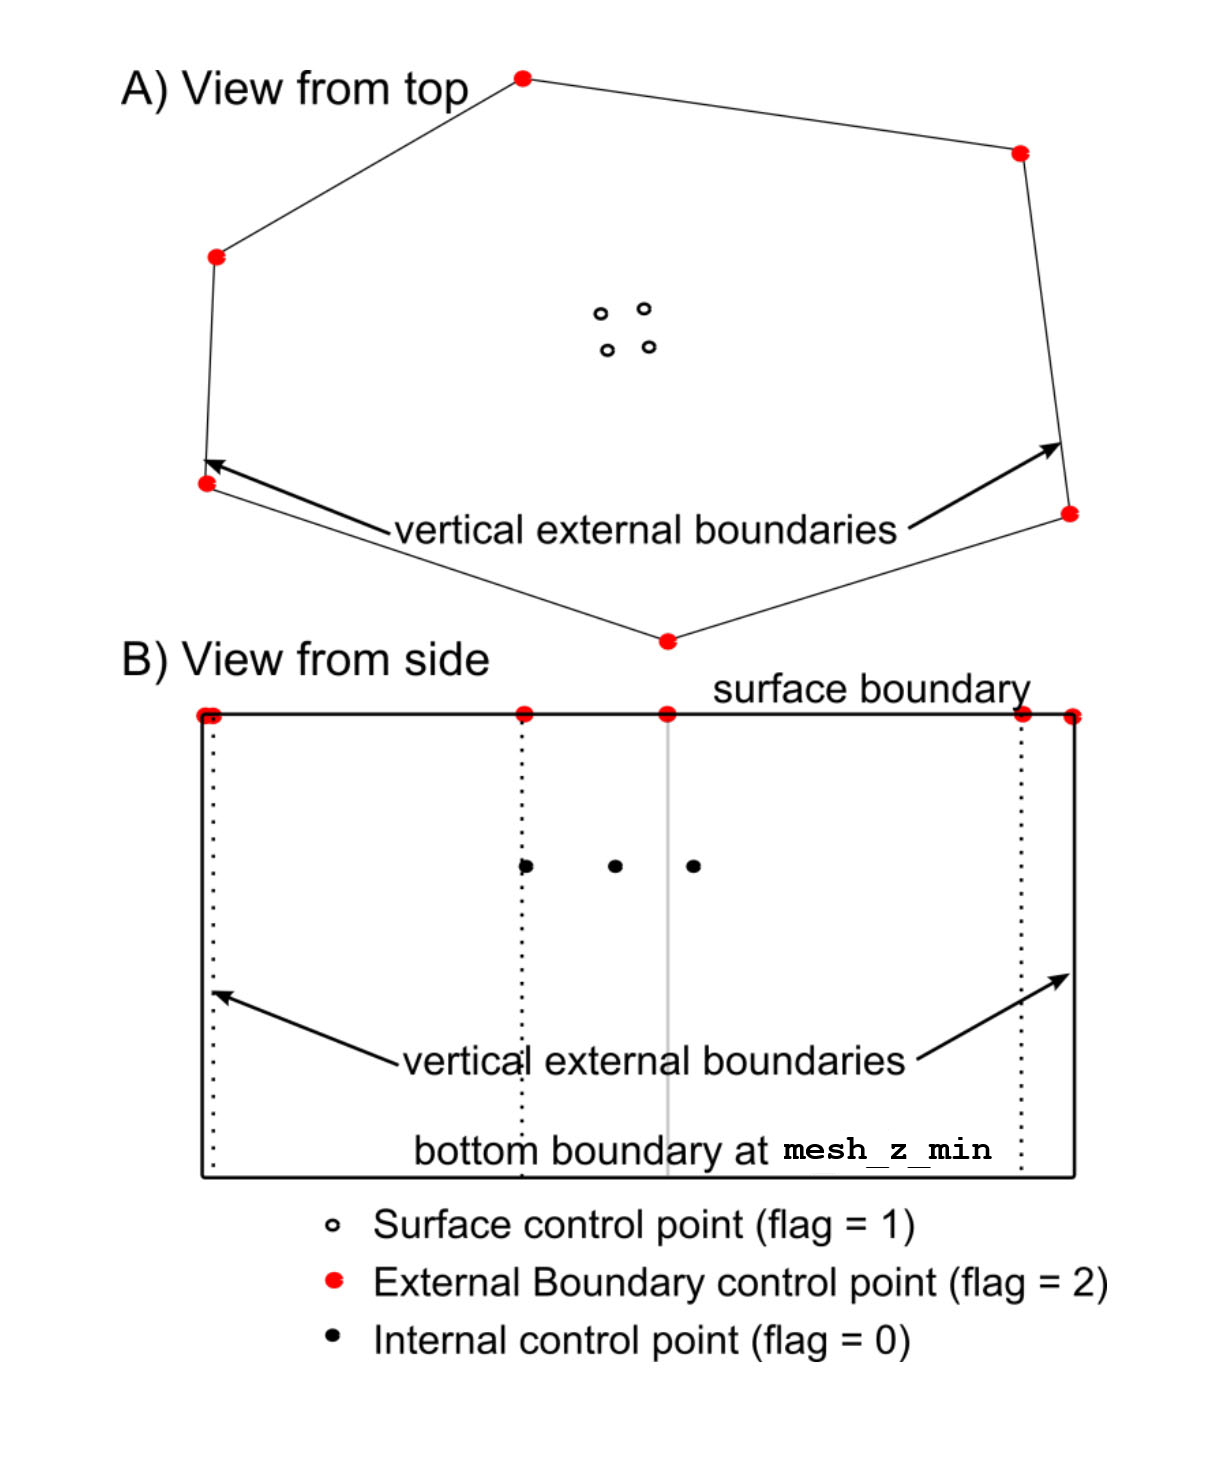
\includegraphics[width=2.6in]{figures/control_point_flags.png} % Adjust width as necessary
    \caption{A diagram showing the three types of control points used to define a mesh.}
    \label{fig:screenshot}
    \end{figure}

    \item[\texttt{nf}] (int)\hfill \\
    The number of internal facets. Facets are polygons used to define zone boundaries. For example, if the user intends to have a rectangular prism-shaped zone, they must define each rectangle that constitutes a face of the prism. A zone must have a closed boundary; thus, any point within the zone must be fully enclosed by facets defined by the user.

    The exception to this rule is if a facet lies entirely on the surface, meaning all its vertices have \texttt{flag[i] = 1}. In this case, E4D automatically generates the facet. This is done to avoid excessive complexity when using E4D with complicated surface topographies.

    For a rectangular prism-shaped zone exposed to the surface, the user must define the four vertical boundaries and the lower boundary. If the zone lies completely beneath the surface, the user must also define the upper boundary.
    
    If two zones share a common facet, it only needs to be defined and counted once.

    \item[\texttt{nv[i]}] (int)\hfill \\
    The total number of vertices defining facet \texttt{i}, e.g., \texttt{nv[i] = 4} for a rectangular facet.

    \item[\texttt{boundary\_id[i]}] (int)\hfill \\
    The boundary ID identifies which boundary facet \texttt{i} belongs to. It is required that \texttt{boundary\_id[i] > 2} as negative numbers, 0, 1, and 2 are reserved in E4D.

    \item[\texttt{v[i][j]}] (int)\hfill \\
    The control point number corresponding to vertex \texttt{j} in facet \texttt{i}.

    \begin{itemize}
        \item Control points must be specified to define a facet such that no segment connecting two consecutive control points crosses any other segment connecting two consecutive control points (i.e., the list of control points should be either clockwise or counter-clockwise). E4D does not check this condition before executing TetGen, and TetGen will fail if this condition is violated.
        \item Each of the points specified must lie in the same plane according to numerical precision, or TetGen will fail.
        \item Do not define facets on any external mesh boundary. E4D will construct these automatically.
        \item The segments of any facet that intersect the surface boundary must be explicitly specified in the plane definition. In other words, any plane segment that intersects the surface boundary must not be defined by the first and last points specified in the facet definition (i.e., the points defining segments on the surface must be listed sequentially in the facet definition).
        \item It is often useful to specify a series of facets that form a closed boundary (thereby forming a zone) whose upper boundary is the surface of the mesh, which is automatically generated by E4D. In this case, E4D must correctly connect the segments of facets intersecting the surface such that those segments define the upper boundary of the zone. To do so, E4D takes the list of control points defining the segments that intersect the surface and connects each point to the next nearest point. With this in mind, it is important to define the facets that intersect the surface in such a manner that E4D correctly connects the surface segments. Attention to this issue is only required for boundaries whose surface intersection forms convex angles.
        \item In the case where the upper boundary of a zone is the surface of the mesh, do not manually specify the facets that make up the upper boundary i.e. do not define any facets where all the control points have \texttt{flag[i] = 1}.
    \end{itemize}

    \item[\texttt{nh}] (int)\hfill \\
    The total number of user-defined holes in the mesh.

    \item[\texttt{xh[i]}] (real)\hfill \\
    The x coordinate of any point within hole \texttt{i}.

    \item[\texttt{yh[i]}] (real)\hfill \\
    The y coordinate of any point within hole \texttt{i}.

    \item[\texttt{zh[i]}] (real)\hfill \\
    The z coordinate of any point within hole \texttt{i}.

    \item[\texttt{nz}] (int)\hfill \\
    The total number of user-defined zones in the mesh.

    \item[\texttt{xz[i]}] (real)\hfill \\
    The x coordinate of any point within zone \texttt{i}.

    \item[\texttt{yz[i]}] (real)\hfill \\
    The y coordinate of any point within zone \texttt{i}.

    \item[\texttt{zz[i]}] (real)\hfill \\
    The z coordinate of any point within zone \texttt{i}.

    \item[\texttt{vol\_max[i]}] (real)\hfill \\
    The maximum volume constraint for all elements within zone \texttt{i}.

    \item[\texttt{sig[i]}] (real)\hfill \\
    The real component of the conductivity of zone \texttt{i} in S/m.

    \item[\texttt{isig[i]}] (real)\hfill \\
    The imaginary component of the conductivity of zone \texttt{i} in S/m. Not required for \texttt{run\_mode = DCR1}.

    \item[\texttt{vis\_flag}] (int)\hfill \\
    Rework needed, set to 0 for the time being.

    \item[\texttt{vis\_loc}] (int)\hfill \\
    Rework needed, set to `none' for the time being.

    \item[\texttt{translate\_flag}] (int)\hfill \\
    Set to 1 to enable E4D automatic translation of the mesh or 0 to disable it. It is recommended to enable translation to minimize potential precision errors. A \hyperref[mesh_trn]{.trn} file will be generated with the corresponding translation values for x, y and z.
\end{description}






\newpage
\subsection{Forward Modelling}

\subsubsection{\texttt{inp} File Format} \label{forward_inp}

\begin{framed}
\noindent \textbf{Important Note:} Must have the \texttt{e4d.inp} file name.
\end{framed}

\begin{framed}
\begin{verbatim}
    run_mode
    mesh_prefix
    srv_filename
    sig_filename
    out_filename
\end{verbatim}
\end{framed}

\begin{description}
    \item[\texttt{run\_mode}] (char)\hfill \\
    Specifies the mode that E4D should run in.
    \begin{itemize}
        \item \texttt{run\_mode = DCR2}: Real potential field and electrical resistivity survey simulation.
        \item \texttt{run\_mode = IP2}: Complex potential field and induced polarisation survey simulation.
    \end{itemize}
    
    \item[\texttt{mesh\_prefix}] (char)\hfill \\
    The prefix of the mesh files from the mesh generation process. These files must be generated beforehand by using the \texttt{DCR1} or \texttt{IP1} run modes. \texttt{mesh\_prefix} is typically based on \texttt{cfg\_filename}

    For example, if \texttt{cfg\_filename = mesh\_prefix.cfg}, then the following files are generated and must be present during forward modelling and inversion.

    \begin{itemize}
        \item \texttt{mesh\_prefix.1.node}
        \item \texttt{mesh\_prefix.1.ele}
        \item \texttt{mesh\_prefix.1.edge}
        \item \texttt{mesh\_prefix.1.face}
        \item \texttt{mesh\_prefix.1.neigh}
        \item \texttt{mesh\_prefix.sig}
        \item \texttt{mesh\_prefix.trn}
    \end{itemize}

    \item[\texttt{srv\_filename}] (char)\hfill \\
    The filename of the \texttt{srv} file. Must have the \texttt{.srv} file extension.

    \item[\texttt{sig\_filename}] (char)\hfill \\
    The filename of the \texttt{sig} file. Must have the \texttt{.sig} file extension.

    \item[\texttt{out\_filename}] (char)\hfill \\
    The filename of the \texttt{out} file. Must have the \texttt{.out} file extension.
\end{description}




\newpage
\subsubsection{\texttt{srv} File Format} \label{forward_srv}

\begin{framed}
\noindent \textbf{Important Note:} Must have the \texttt{.srv} file extension.
\end{framed}

\begin{framed}
\begin{verbatim}
    ne
    1 x[1] y[1] z[1] flag[1]
    2 x[2] y[2] z[2] flag[2]
    ...
    ne x[ne] y[ne] z[ne] flag[ne]

    nm
\end{verbatim}

\begingroup
\scriptsize
\begin{verbatim}
      1 c1[1] c2[1] p1[1] p2[1] dcr_obs[1] dcr_sd[1] ip_obs[1] ip_sd[1]
      2 c1[2] c2[2] p1[2] p2[2] dcr_obs[2] dcr_sd[2] ip_obs[2] ip_sd[2]
      ...
      nm c1[nm] c2[nm] p1[nm] p2[nm] dcr_obs[nm] dcr_sd[nm] ip_obs[nm] ip_sd[nm]
\end{verbatim}
\endgroup
\end{framed}

\begin{description}
    \item[\texttt{ne}] (int)\hfill \\
    The total number of unique electrodes in the survey.
    
    \item[\texttt{x[i]}] (real)\hfill \\
    The x coordinate of electrode \texttt{i}.

    \item[\texttt{y[i]}] (real)\hfill \\
    The y coordinate of electrode \texttt{i}.

    \item[\texttt{z[i]}] (real)\hfill \\
    The z coordinate of electrode \texttt{i}.

    \item[\texttt{flag[i]}] (int)\hfill \\
    The flag of electrode \texttt{i}:
    \begin{itemize}
        \item \texttt{flag[i] = 1}: Surface electrode.
        \item \texttt{flag[i] = 0}: Sub-surface electrode.
    \end{itemize}
    
    \item[\texttt{nm}] (int)\hfill \\
    The total number of survey measurements.

    \item[\texttt{c1[i]}] (int)\hfill \\
    The electrode index of the positive current electrode in measurement \texttt{i}.

    \item[\texttt{c2[i]}] (int)\hfill \\
    The electrode index of the negative current electrode in measurement \texttt{i}.

    \item[\texttt{p1[i]}] (int)\hfill \\
    The electrode index of the positive potential electrode in measurement \texttt{i}.

    \item[\texttt{p2[i]}] (int)\hfill \\
    The electrode index of the negative potential electrode in measurement \texttt{i}.

    \item[\texttt{dcr\_obs[i]}] (real)\hfill \\
    The observed transfer resistance of measurement \texttt{i} in ohms. For forward modelling, use an arbitrary placeholder value.

    \item[\texttt{dcr\_sd[i]}] (real)\hfill \\
    The transfer resistance standard deviation of measurement \texttt{i} in ohms. For forward modelling, use an arbitrary placeholder value.

    \item[\texttt{ip\_obs[i]}] (real)\hfill \\
    The observed phase of measurement \texttt{i} in radians. For forward modelling, use an arbitrary placeholder value. Not required for \texttt{run\_mode = DCR2}.

    \item[\texttt{ip\_sd[i]}] (real)\hfill \\
    The phase standard deviation of measurement \texttt{i} in radians. For forward modelling, use an arbitrary placeholder value. Not required for \texttt{run\_mode = DCR2}.
\end{description}


\newpage
\subsubsection{\texttt{sig} File Format} \label{forward_sig}

\begin{framed}
\noindent \textbf{Important Note:} A \texttt{sig} file is created during the mesh generation stage based on the defined zone properties. Often, it is adequate to use this, although the user may choose to define their own.
\end{framed}

\begin{framed}
\begin{verbatim}
    nel
    1 sigma[1] isigma[1]
    2 sigma[2] isigma[2]
    ...
    nel sigma[nel] isigma[nel]
\end{verbatim}
\end{framed}

\begin{description}
    \item[\texttt{nel}] (int)\hfill \\
    The total number of elements in the mesh.
    
    \item[\texttt{sigma[i]}] (real)\hfill \\
    The real conductivity of element \texttt{i} in S/m.

    \item[\texttt{isigma[i]}] (real)\hfill \\
    The imaginary conductivity of element \texttt{i} in S/m.  Not required for \texttt{run\_mode = DCR2}.
\end{description}


\newpage
\subsubsection{\texttt{out} File Format} \label{forward_out}

\begin{framed}
\noindent \textbf{Important Note:} Must have the \texttt{.out} file extension.
\end{framed}

\begin{framed}
\begin{verbatim}
    residual_flag
    residual_prefix
    npot
    pot[1]
    pot[2]
    ...
    pot[npot]
\end{verbatim}
\end{framed}

\begin{description}
    \item[\texttt{residual\_flag}] (int)\hfill \\
    Determines whether or not to output a residual data file for the given model. For forward modelling, the observed data will be the placeholder values specified in the \texttt{srv} file and the predicted values will be the forward response.
    \begin{itemize}
        \item \texttt{residual\_flag = 0}: Does not output a residual data file.
        \item \texttt{residual\_flag = 1}: Outputs a residual data file.
    \end{itemize}
    
    \item[\texttt{residual\_prefix}] (char)\hfill \\
    The prefix of the residual data file. For forward modelling, the filename will be \texttt{residual\_prefix.txt}.
    
    \item[\texttt{npot}] (int)\hfill \\
    The number of potential distribution files to output.

    \item[\texttt{pot[i]}] (int)\hfill \\
    The index of measurement \texttt{i} from the \texttt{srv} file for which to output the potential distribution.
\end{description}


\newpage
\subsection{Inversion}

\subsubsection{\texttt{inp} File Format} \label{inversion_inp}

\begin{framed}
\noindent \textbf{Important Note:} Must have the \texttt{e4d.inp} file name.
\end{framed}

\begin{framed}
\begin{verbatim}
    run_mode
    mesh_prefix
    srv_filename
    initial_model
    out_filename
    dcr_inv_filename ip_inv_filename
    reference_model
\end{verbatim}
\end{framed}

\begin{description}
    \item[\texttt{run\_mode}] (char)\hfill \\
    Specifies the mode that E4D should run in.
    \begin{itemize}
        \item \texttt{run\_mode = DCR3}: Electrical resistivity inversion for a single survey.
        \item \texttt{run\_mode = IP3}: Complex resistivity survey for a single survey.
    \end{itemize}
    
    \item[\texttt{mesh\_prefix}] (char)\hfill \\
    The prefix of the mesh files from the mesh generation process. These files must be generated beforehand by using the \texttt{DCR1} or \texttt{IP1} run modes. \texttt{mesh\_prefix} is typically based on \texttt{cfg\_filename}

    For example, if \texttt{cfg\_filename = mesh\_prefix.cfg}, then the following files are generated and must be present during forward modelling and inversion.

    \begin{itemize}
        \item \texttt{mesh\_prefix.1.node}
        \item \texttt{mesh\_prefix.1.ele}
        \item \texttt{mesh\_prefix.1.edge}
        \item \texttt{mesh\_prefix.1.face}
        \item \texttt{mesh\_prefix.1.neigh}
        \item \texttt{mesh\_prefix.sig}
        \item \texttt{mesh\_prefix.trn}
    \end{itemize}

    \item[\texttt{srv\_filename}] (char)\hfill \\
    The filename of the \texttt{srv} file. Must have the \texttt{.srv} file extension.

    \item[\texttt{initial\_model}] (char)\hfill \\
    \begin{itemize}
        \item \texttt{initial\_model = `average'}: Sets the initial model to use the average apparent conductivity and apparent phase.
        \item \texttt{initial\_model = `sig\_file\_name'}: Alternatively, a \texttt{sig\_filename} can be specified.
    \end{itemize}

    \item[\texttt{out\_filename}] (char)\hfill \\
    The filename of the \texttt{out} file. Must have the \texttt{.out} file extension.

    \item[\texttt{dc\_inv\_filename}] (char)\hfill \\
    The filename of the \texttt{dc\_inv} file. Must have the \texttt{.inv} file extension.

    \item[\texttt{ip\_inv\_filename}] (char)\hfill \\
    The filename of the \texttt{ip\_inv} file. Must have the \texttt{.inv} file extension. Not required for \texttt{run\_mode = DCR3}.

    \item[\texttt{reference\_model}] (char)\hfill \\
    \begin{itemize}
        \item \texttt{reference\_model = `none'}: Set to none unless the user requires inversion constraints based on a reference model.
        \item \texttt{reference\_model = `sig\_file\_name'}: Alternatively, a \texttt{sig\_filename} can be specified.
    \end{itemize}
\end{description}




\newpage
\subsubsection{\texttt{srv} File Format} \label{forward_srv}

\begin{framed}
\noindent \textbf{Important Note:} Must have the \texttt{.srv} file extension.
\end{framed}

\begin{framed}
\begin{verbatim}
    ne
    1 x[1] y[1] z[1] flag[1]
    2 x[2] y[2] z[2] flag[2]
    ...
    ne x[ne] y[ne] z[ne] flag[ne]

    nm
\end{verbatim}

\begingroup
\scriptsize
\begin{verbatim}
      1 c1[1] c2[1] p1[1] p2[1] dcr_obs[1] dcr_sd[1] ip_obs[1] ip_sd[1]
      2 c1[2] c2[2] p1[2] p2[2] dcr_obs[2] dcr_sd[2] ip_obs[2] ip_sd[2]
      ...
      nm c1[nm] c2[nm] p1[nm] p2[nm] dcr_obs[nm] dcr_sd[nm] ip_obs[nm] ip_sd[nm]
\end{verbatim}
\endgroup
\end{framed}

\begin{description}
    \item[\texttt{ne}] (int)\hfill \\
    The total number of unique electrodes in the survey.
    
    \item[\texttt{x[i]}] (real)\hfill \\
    The x coordinate of electrode \texttt{i}.

    \item[\texttt{y[i]}] (real)\hfill \\
    The y coordinate of electrode \texttt{i}.

    \item[\texttt{z[i]}] (real)\hfill \\
    The z coordinate of electrode \texttt{i}.

    \item[\texttt{flag[i]}] (int)\hfill \\
    The flag of electrode \texttt{i}:
    \begin{itemize}
        \item \texttt{flag[i] = 1}: Surface electrode.
        \item \texttt{flag[i] = 0}: Sub-surface electrode.
    \end{itemize}
    
    \item[\texttt{nm}] (int)\hfill \\
    The total number of survey measurements.

    \item[\texttt{c1[i]}] (int)\hfill \\
    The electrode index of the positive current electrode in measurement \texttt{i}.

    \item[\texttt{c2[i]}] (int)\hfill \\
    The electrode index of the negative current electrode in measurement \texttt{i}.

    \item[\texttt{p1[i]}] (int)\hfill \\
    The electrode index of the positive potential electrode in measurement \texttt{i}.

    \item[\texttt{p2[i]}] (int)\hfill \\
    The electrode index of the negative potential electrode in measurement \texttt{i}.

    \item[\texttt{dcr\_obs[i]}] (real)\hfill \\
    The observed transfer resistance of measurement \texttt{i} in ohms.

    \item[\texttt{dcr\_sd[i]}] (real)\hfill \\
    The transfer resistance standard deviation of measurement \texttt{i} in ohms.

    \item[\texttt{ip\_obs[i]}] (real)\hfill \\
    The observed phase of measurement \texttt{i} in radians. Not required for \texttt{run\_mode = DCR3}.

    \item[\texttt{ip\_sd[i]}] (real)\hfill \\
    The phase standard deviation of measurement \texttt{i} in radians. Not required for \texttt{run\_mode = DCR3}.
\end{description}


\newpage
\subsubsection{\texttt{out} File Format} \label{forward_out}

\begin{framed}
\noindent \textbf{Important Note:} Must have the \texttt{.out} file extension.
\end{framed}

\begin{framed}
\begin{verbatim}
    residual_flag
    residual_prefix
    npot
    pot[1]
    pot[2]
    ...
    pot[npot]
\end{verbatim}
\end{framed}

\begin{description}
    \item[\texttt{residual\_flag}] (int)\hfill \\
    Determines whether or not to output a residual data file for the given model.
    \begin{itemize}
        \item \texttt{residual\_flag = 0}: Does not output a residual data file.
        \item \texttt{residual\_flag = 1}: Outputs a residual data file.
    \end{itemize}
    
    \item[\texttt{residual\_prefix}] (char)\hfill \\
    The prefix of the residual data file. For forward modelling, the filename will be \texttt{residual\_prefix.txt}.
    
    \item[\texttt{npot}] (int)\hfill \\
    The number of potential distribution files to output.

    \item[\texttt{pot[i]}] (int)\hfill \\
    The index of measurement \texttt{i} from the \texttt{srv} file for which to output the potential distribution.
\end{description}


\newpage
\subsubsection{\texttt{inv} File Format (DCR)} \label{inversion_dc}

\begin{framed}
\noindent \textbf{Important Note:} Must have the \texttt{.inv} file extension.
\end{framed}

\begin{framed}
\begin{verbatim}
    nc

    zone[1]
    struct_met[1] wx[1] wy[1] wz[1]
    f[1] mn[1] sd[1]
    nl[1] link[1][1] link[1][2] ... link[1][nl]
    ref_value
    ref_weight

    zone[2]
    struct_met[2] wx[2] wy[2] wz[2]
    f[2] mn[2] sd[2]
    nl[2] link[2][1] link[2][2] ... link[2][nl]
    ref_value[2]
    ref_weight[2]

    ...

    zone[nc]
    struct_met[nc] wx[nc] wy[nc] wz[nc]
    f[nc] mn[nc] sd[nc]
    nl[nc] link[nc][1] link[nc][2] ... link[nc][nl]
    ref_value[nc]
    ref_weight[nc]

    initial_beta min_decrease beta_reduction
    chi2_target
    min_iter max_iter
    min_sig max_sig
    beta_mode
    outlier_mode outlier_sd
\end{verbatim}
\end{framed}



\begin{description}
    \item[\texttt{nc}] (int)\hfill \\
     The total number of constraint blocks. Each zone in the mesh is considered a constraint block and should have at least one assignment.
    
    \item[\texttt{zone[i]}] (int)\hfill \\
     The zone number for which this constraint block applies.
    
    \item[\texttt{struct\_met[i]}] (int)\hfill \\
     The structural metric to use for constraint \texttt{i}. For more details, see section \ref{structural_metrics}.

    \item[\texttt{wx[i]}] (real)\hfill \\
    The relative weighting of this structure metric in the x direction. This is not used by every structural metric and is ignored if not used. However, they must be present in this file.

    \item[\texttt{wy[i]}] (real)\hfill \\
    The relative weighting of this structure metric in the y direction. This is not used by every structural metric and is ignored if not used. However, they must be present in this file.

    \item[\texttt{wz[i]}] (real)\hfill \\
    The relative weighting of this structure metric in the z direction. This is not used by every structural metric and is ignored if not used. However, they must be present in this file.

    \item[\texttt{f[i]}] (int)\hfill \\
     The weighting function to use for constraint \texttt{i}. For more details, see section \ref{weighting_functions}.

    \item[\texttt{mn[i]}] (real)\hfill \\
     The mean of the weighting function in natural log space.

     \item[\texttt{sd[i]}] (real)\hfill \\
     The standard deviation of the weighting function in natural log space.

    \item[\texttt{ref\_value[i]}] (real/char)\hfill \\
     The reference value used for this constraint block. If specified as ``REF" or ``Ref" or ``ref", then the reference model specified in \texttt{inp} file is used to provide the reference values for this constraint block.

     \item[\texttt{ref\_weight[i]}] (real)\hfill \\
     The relative weight applied to the regularisation constraints specified in this block.

     \item[\texttt{initial\_beta}] (real)\hfill \\
     The global constraint weighting value at the beginning of the inversion, and controls the importance the inversion places on enforcing the model constraints in comparison to fitting the data. This parameter is either held constant or automatically reduced by E4D during the inversion when required to reduce the misfit between measured and simulated data.

    \item[\texttt{min\_decrease}] (real)\hfill \\
     The minimum fractional decrease in the objective function between outer iterations that may occur before beta is reduced. A conservative value for is \texttt{min\_decrease = 0.05}. Larger values will generally decrease time to convergence, but may also provide solutions that violate the model constraints more than what is necessary to appropriately fit the data.

     \item[\texttt{beta\_reduction}] (real)\hfill \\
     The beta reduction factor. If the fractional decrease in the objective function between outer iterations is less than or equal to \texttt{min\_decrease}, then beta is reduced by a factor of \texttt{beta\_reduction} for the next iteration. A conservative value is \texttt{beta\_reduction = 0.5}.

     \item[\texttt{chi2\_target}] (real)\hfill \\
     The normalised $\chi^2$ value at which the inversion is considered to have converged. In the absence of modelling errors and accurately specified data standard deviations, $\chi^2$ should reach a value of 1.0 at convergence.

     \item[\texttt{min\_iter}] (int)\hfill \\
     The minimum number of inner iterations (i.e. CGLS iterations) to execute before updating the solution. Recommended value is \texttt{min\_iter = 30}.

     \item[\texttt{max\_iter}] (int)\hfill \\
     The minimum number of inner iterations (i.e. CGLS iterations) to execute before updating the solution. Recommended value is \texttt{max\_iter = 50}.

     \item[\texttt{min\_sig}] (real)\hfill \\
     The minimum conductivity value allowed by the inversion. These values do not constrain the inversion, and are only provided as a safety mechanism to ensure the forward solution remains stable. Maximum and minimum conductivity constraints should be specified in the constraints block.

     \item[\texttt{max\_sig}] (real)\hfill \\
     The maximum conductivity value allowed by the inversion. These values do not constrain the inversion, and are only provided as a safety mechanism to ensure the forward solution remains stable. Maximum and minimum conductivity constraints should be specified in the constraints block.

     \item[\texttt{beta\_mode}] (int)\hfill \\
    \begin{itemize}
        \item \texttt{beta\_mode = 2}: Beta reduces as the inversion progresses.
        \item \texttt{beta\_mode = 3}: Beta remains constant throughout the inversion.
    \end{itemize}

    \item[\texttt{outlier\_mode}] (int)\hfill \\
    \begin{itemize}
        \item \texttt{outlier\_mode = 0}: No outlier removal
        \item \texttt{outlier\_mode = 1}: Remove outlier datum from the current inversion iteration.
    \end{itemize}

    \item[\texttt{outlier\_sd}] (int)\hfill \\
    Specifies the outlier removal standard deviation. If the weighted residual error of any datum is greater than \texttt{outlier\_sd} standard deviations from the mean weighted residual error and \texttt{outlier\_mode = 1}, then that datum is not used to constrain the inversion in next iteration. Recommended to set \texttt{outlier\_sd = 3}.

\end{description}


\newpage
\subsubsection{\texttt{inv} File Format (IP)} \label{inversion_ip}

\begin{framed}
\noindent \textbf{Important Note:} Must have the \texttt{.inv} file extension. Not required for \texttt{run\_mode = DCR3}
\end{framed}

\begin{framed}
\begin{verbatim}
    nc

    zone[1]
    struct_met[1] wx[1] wy[1] wz[1]
    f[1] mn[1] sd[1]
    nl[1] link[1][1] link[1][2] ... link[1][nl]
    ref_value[1]
    ref_weight[1]

    zone[2]
    struct_met[2] wx[2] wy[2] wz[2]
    f[2] mn[2] sd[2]
    nl[2] link[2][1] link[2][2] ... link[2][nl]
    ref_value[2]
    ref_weight[2]

    ...

    zone[nc]
    struct_met[nc] wx[nc] wy[nc] wz[nc]
    f[nc] mn[nc] sd[nc]
    nl[nc] link[nc][1] link[nc][2] ... link[nc][nl]
    ref_value[nc]
    ref_weight[nc]

    initial_beta min_decrease beta_reduction
    chi2_target
    min_iter max_iter
    min_phase max_phase
    beta_mode
    outlier_mode outlier_sd
\end{verbatim}
\end{framed}



\begin{description}
    \item[\texttt{nc}] (int)\hfill \\
     The total number of constraint blocks. Each zone in the mesh is considered a constraint block and should have at least one assignment.
    
    \item[\texttt{zone[i]}] (int)\hfill \\
     The zone number for which this constraint block applies.
    
    \item[\texttt{struct\_met[i]}] (int)\hfill \\
     The structural metric to use for constraint \texttt{i}. For more details, see section \ref{structural_metrics}.

    \item[\texttt{wx[i]}] (real)\hfill \\
    The relative weighting of this structure metric in the x direction. This is not used by every structural metric and is ignored if not used. However, they must be present in this file.

    \item[\texttt{wy[i]}] (real)\hfill \\
    The relative weighting of this structure metric in the y direction. This is not used by every structural metric and is ignored if not used. However, they must be present in this file.

    \item[\texttt{wz[i]}] (real)\hfill \\
    The relative weighting of this structure metric in the z direction. This is not used by every structural metric and is ignored if not used. However, they must be present in this file.

    \item[\texttt{f[i]}] (int)\hfill \\
     The weighting function to use for constraint \texttt{i}.For more details, see section \ref{weighting_functions}.

    \item[\texttt{mn[i]}] (real)\hfill \\
     The mean of the weighting function in natural log space.

     \item[\texttt{sd[i]}] (real)\hfill \\
     The standard deviation of the weighting function in natural log space.

    \item[\texttt{ref\_value[i]}] (real/char)\hfill \\
     The reference value used for this constraint block. If specified as ``REF" or ``Ref" or ``ref", then the reference model specified in \texttt{inp} file is used to provide the reference values for this constraint block.

     \item[\texttt{ref\_weight[i]}] (real)\hfill \\
     The relative weight applied to the regularisation constraints specified in this block.

     \item[\texttt{initial\_beta}] (real)\hfill \\
     The global constraint weighting value at the beginning of the inversion, and controls the importance the inversion places on enforcing the model constraints in comparison to fitting the data. This parameter is either held constant or automatically reduced by E4D during the inversion when required to reduce the misfit between measured and simulated data.

    \item[\texttt{min\_decrease}] (real)\hfill \\
     The minimum fractional decrease in the objective function between outer iterations that may occur before beta is reduced. A conservative value for is \texttt{min\_decrease = 0.05}. Larger values will generally decrease time to convergence, but may also provide solutions that violate the model constraints more than what is necessary to appropriately fit the data.

     \item[\texttt{beta\_reduction}] (real)\hfill \\
     The beta reduction factor. If the fractional decrease in the objective function between outer iterations is less than or equal to \texttt{min\_decrease}, then beta is reduced by a factor of \texttt{beta\_reduction} for the next iteration. A conservative value is \texttt{beta\_reduction = 0.5}.

     \item[\texttt{chi2\_target}] (real)\hfill \\
     The normalised $\chi^2$ value at which the inversion is considered to have converged. In the absence of modelling errors and accurately specified data standard deviations, $\chi^2$ should reach a value of 1.0 at convergence.

     \item[\texttt{min\_iter}] (int)\hfill \\
     The minimum number of inner iterations (i.e. CGLS iterations) to execute before updating the solution. Recommended value is \texttt{min\_iter = 30}.

     \item[\texttt{max\_iter}] (int)\hfill \\
     The minimum number of inner iterations (i.e. CGLS iterations) to execute before updating the solution. Recommended value is \texttt{max\_iter = 50}.

     \item[\texttt{min\_phase}] (real)\hfill \\
     The minimum phase value allowed by the inversion. These values do not constrain the inversion, and are only provided as a safety mechanism to ensure the forward solution remains stable. Maximum and minimum phase constraints should be specified in the constraints block.

     \item[\texttt{max\_phase}] (real)\hfill \\
     The maximum phase value allowed by the inversion. These values do not constrain the inversion, and are only provided as a safety mechanism to ensure the forward solution remains stable. Maximum and minimum phase constraints should be specified in the constraints block.

     \item[\texttt{beta\_mode}] (int)\hfill \\
    \begin{itemize}
        \item \texttt{beta\_mode = 2}: Beta reduces as the inversion progresses.
        \item \texttt{beta\_mode = 3}: Beta remains constant throughout the inversion.
    \end{itemize}

    \item[\texttt{outlier\_mode}] (int)\hfill \\
    \begin{itemize}
        \item \texttt{outlier\_mode = 0}: No outlier removal
        \item \texttt{outlier\_mode = 1}: Remove outlier datum from the current inversion iteration.
    \end{itemize}

    \item[\texttt{outlier\_sd}] (int)\hfill \\
    Specifies the outlier removal standard deviation. If the weighted residual error of any datum is greater than \texttt{outlier\_sd} standard deviations from the mean weighted residual error and \texttt{outlier\_mode = 1}, then that datum is not used to constrain the inversion in next iteration. Recommended to set \texttt{outlier\_sd = 3}.

\end{description}


\newpage
\section{Miscellaneous File Formats}

\subsubsection{\texttt{node/ele/edge/face/neigh} File Format} \label{mesh_files}

These files are created by TetGen during the \texttt{DCR1} or \texttt{IP1} run modes. They define the mesh and are required for both forward modelling and inversion.

If \texttt{cfg\_filename = mesh\_prefix.cfg}, then the following files are generated:

\begin{itemize}
    \item \texttt{mesh\_prefix.1.node}
    \item \texttt{mesh\_prefix.1.ele}
    \item \texttt{mesh\_prefix.1.edge}
    \item \texttt{mesh\_prefix.1.face}
    \item \texttt{mesh\_prefix.1.neigh}
\end{itemize}

A detailed description of each mesh file format is available in the TetGen manual \cite{10.1145/2629697}.


\newpage
\subsubsection{\texttt{trn} File Format} \label{mesh_trn}

\begin{framed}
\noindent \textbf{Important Note:} A \texttt{trn} file is created during the mesh generation contains the x,y and z coordinate translations used internally by E4D.
\end{framed}

\begin{framed}
\begin{verbatim}
   delta_x delta_y delta_z
\end{verbatim}
\end{framed}

\begin{description}
    \item[\texttt{delta\_x}] (real)\hfill \\
    The translation of the mesh in the x-direction in meters.

    \item[\texttt{delta\_y}] (real)\hfill \\
    The translation of the mesh in the y-direction in meters.

    \item[\texttt{delta\_z}] (real)\hfill \\
    The translation of the mesh in the z-direction in meters.
\end{description}





\section{IP Inversion Tutorial}

\begin{framed}
\noindent \textbf{Important Note:} The required input files for this tutorial are located in: \texttt{/tutorial/two\_blocks/}
\end{framed}

This section provides a step-by-step tutorial for building a synthetic model, calculating the forward response, and inverting the data with smoothness constraints to attempt the recovery of the original model. Through this tutorial, users will gain practical experience with the process of forward modelling and inversion using E4D.

The synthetic model consists of a flat surface with two buried blocks, each measuring 200 m × 200 m × 200 m. The model parameters are as follows:

\begin{itemize}
    \item \textbf{Background:} 
    \begin{itemize}
        \item Resistivity: 500 ohm-m
        \item Phase: 1 mrad
    \end{itemize}
    \item \textbf{Block 1:} 
    \begin{itemize}
        \item Resistivity: 5 ohm-m
        \item Phase: 100 mrad
    \end{itemize}
    \item \textbf{Block 2:} 
    \begin{itemize}
        \item Resistivity: 5000 ohm-m
        \item Phase: 10 mrad
    \end{itemize}
\end{itemize}

\begin{figure}[H]
\centering
\fbox{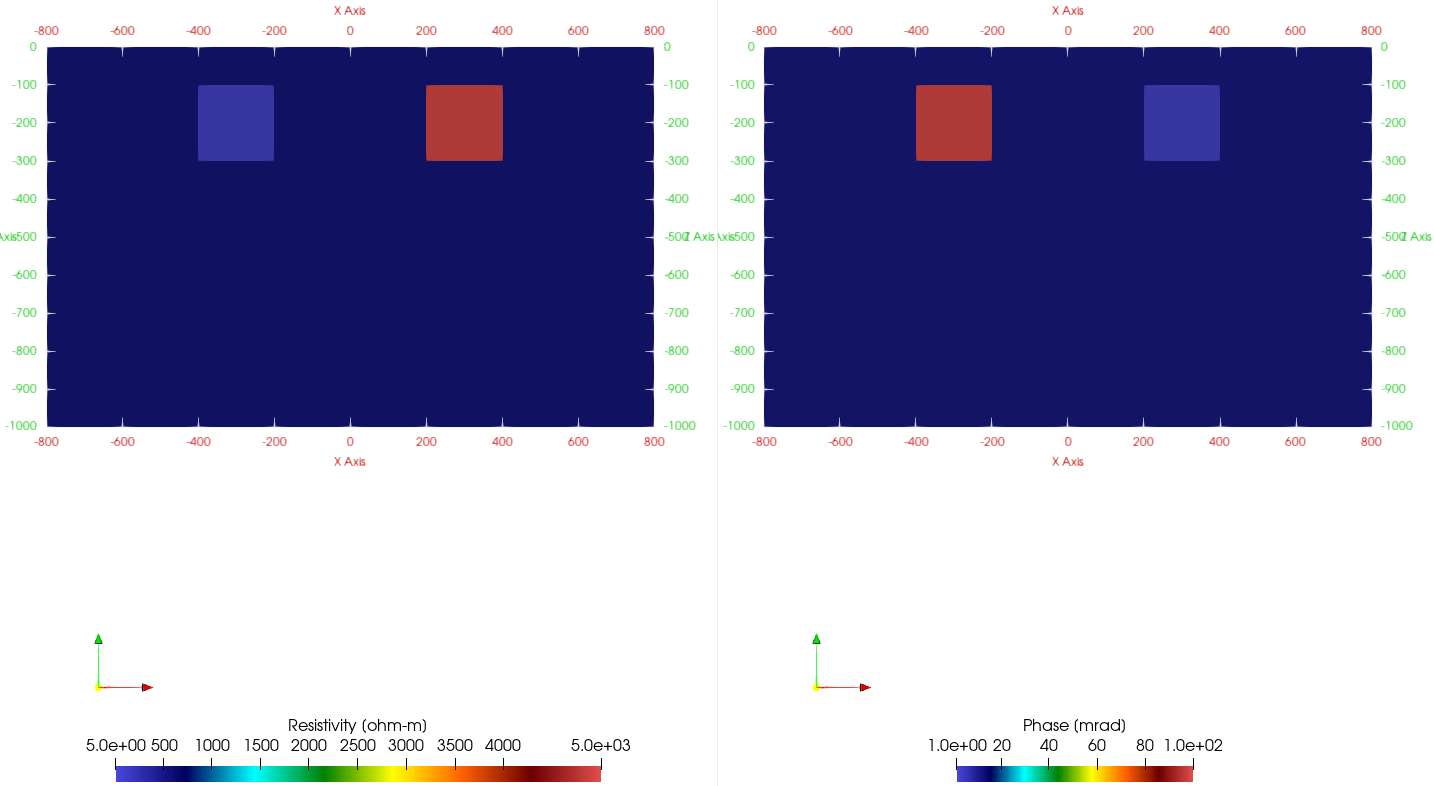
\includegraphics[width=7.0in]{figures/two_blocks_dcr_ip.png}}
\caption{Synthetic model section view.}
\label{fig:model}
\end{figure}



\subsection{Preliminary Setup} \label{prelim}

It is strongly recommended to compile E4D, TetGen, and Triangle using the Intel oneAPI compilers (see Section \ref{install} for detailed instructions). To enable support for oneAPI, it is necessary to configure the environment variables accordingly.

Begin by opening a terminal in the intended working directory and sourcing the oneAPI environment setup script:

\begin{verbatim}
source /opt/intel/oneapi/setvars.sh
\end{verbatim}

Next, configure the MPI communication fabric by setting the following environment variable:

\begin{verbatim}
export I_MPI_FABRICS=shm
\end{verbatim}

Finally, add the directory containing the required executables to your system’s PATH:

\begin{verbatim}
export PATH="$PATH:../E4D-HR/bin"
\end{verbatim}

\subsection{Forward IP1}

\subsubsection{Input Files}

In the \texttt{/two\_blocks/forward\_IP1/} directory, you will find two key files:

\begin{itemize}
    \item \texttt{e4d.inp}
    \item \texttt{two\_blocks.cfg}
\end{itemize}

The \texttt{e4d.inp} file instructs E4D to run in the specified mode, which in this case is IP mesh generation, or \texttt{IP1}. The \texttt{two\_blocks.cfg} file contains the necessary information to build the mesh, which we will examine closely in this section.

Examining \texttt{two\_blocks.cfg} line by line, we observe the following standard options:

\begin{itemize}
    \item \texttt{mesh\_qual = 1.3}: Ensures that highly irregularly shaped tetrahedral elements are avoided, as these are commonly associated with poor numerical accuracy.
    \item \texttt{mesh\_vol\_max = 1e18}: While this value may seem excessively large, it is acceptable since small element sizes are not required far away from potential sources.
    \item \texttt{tetgen\_flag = 1}: Instructs TetGen to build the mesh.
    \item \texttt{tetgen\_path = tetgen}: Specifies the path to the TetGen executable, assuming it has been added to the system's PATH environment variable as described in Section \ref{prelim}.
    \item \texttt{triangle\_path = triangle}: Specifies the path to the Triangle executable, assuming it has been added to the system's PATH environment variable as described in Section \ref{prelim}.
\end{itemize}

Moving on to the control point definitions, there are 124 points defined in the following order:

\begin{itemize}
    \item The 4 surface boundary points.
    \item The 8 vertices of zone 1, which is a 1600 m × 1200 m × 2000 m rectangular prism.
    \item The 8 vertices of zone 2, which is a 200 m × 200 m × 200 m cube.
    \item The 8 vertices of zone 3, which is also a 200 m × 200 m × 200 m cube.
    \item 48 electrode locations.
    \item 48 electrode refinement points, located 5 m below each electrode to enforce smaller element sizes, thereby improving numerical accuracy during modelling.
\end{itemize}

Next, we define 17 facets in the \texttt{two\_blocks.cfg} file. The first 5 facets correspond to the 4 vertical faces and the lower face of the boundary that encloses zone 1. It’s important to note that the upper face is not specified because all vertices of the upper face have \texttt{flag = 1}, allowing E4D to automatically handle this case.

The following 6 facets correspond to the 6 faces of the first block (zone 2), listed in the following order: upper, vertical, and lower. In this instance, all 6 faces are specified because the block is entirely below the surface.

The final 6 facets correspond to the 6 faces of the second block (zone 3), listed in the same order: upper, vertical, and lower.

Continuing on, we observe that there are no defined holes in this mesh, which is typical for most configurations.

Next, we define 4 zones within the mesh: the background, the first block, the second block, and the remainder of the mesh.

Each zone is defined by specifying a point that lies within it. We also specify the maximum element size for each zone. Notably, zone 4 (the remainder of the mesh) has a larger maximum element size because elements in this zone are located far from potential sources, and therefore, do not require as much refinement. Additionally, we define the real and imaginary conductivity for each zone, which will be used in the modelling process.

Finally, we set the following parameters:

\begin{itemize}
    \item \texttt{vis\_flag = 0}: Disables visualisation output.
    \item \texttt{vis\_loc = none}: Specifies no visualisation location.
    \item \texttt{translate\_flag = 0}: Disables any translation of the mesh.
\end{itemize}

Understanding the concept of zones in E4D is crucial, especially when it comes to defining facets. It is recommended to take the time to thoroughly examine the \texttt{two\_blocks.cfg} file.

\subsubsection{Generating the Mesh with the IP1 mode}

To begin the mesh generation process, ensure that your working directory contains the following files:

\begin{itemize}
    \item \texttt{e4d.inp}
    \item \texttt{two\_blocks.cfg}
\end{itemize}

Verify that all steps outlined in Section \ref{prelim} have been completed within the current terminal environment.

To execute the process, use the following command:

\begin{verbatim}
mpirun -np n e4d
\end{verbatim}

Here, \texttt{n} represents the number of processors you wish to utilise for parallel execution of E4D.

Upon successful execution, the following files should be present in your working directory:

\begin{itemize}
    \item \texttt{two\_blocks.1.node}
    \item \texttt{two\_blocks.1.ele}
    \item \texttt{two\_blocks.1.edge}
    \item \texttt{two\_blocks.1.face}
    \item \texttt{two\_blocks.1.neigh}
    \item \texttt{two\_blocks.trn}
    \item \texttt{two\_blocks.sig}
\end{itemize}

\subsection{Forward Model} \label{two_blocks_forward}

\subsubsection{Input Files}

In the \texttt{/two\_blocks/forward\_IP1/} directory, you will find three key files:

\begin{itemize}
    \item \texttt{e4d.inp}
    \item \texttt{dummy.srv}
    \item \texttt{e4d.out}
\end{itemize}

The file to pay particular attention to is \texttt{dummy.srv}. This file contains the locations of each electrode, followed by the electrode configuration for each measurement that will be used to calculate the forward response. You might wonder why observation and error values are included in this file, even though the forward model has not yet been calculated. These are placeholder or dummy values, which are required by the process but have no effect on the forward modelling itself. Familiarise yourself with this file format—more details can be found in Section \ref{forward_srv}—as the \texttt{srv} file format is what you will need to convert your survey data into when inverting real field data. 

The \texttt{e4d.out} file contains standard settings and does not include any additional options to export the potential distribution.

\subsubsection{Calculating a Forward Model with the IP2 mode}

To initiate the forward modelling process, ensure that your working directory contains the following files:

\begin{itemize}
    \item \texttt{e4d.inp}
    \item \texttt{dummy.srv}
    \item \texttt{e4d.out}
\end{itemize}

Additionally, include the mesh files generated in the previous section:

\begin{itemize}
    \item \texttt{two\_blocks.1.node}
    \item \texttt{two\_blocks.1.ele}
    \item \texttt{two\_blocks.1.edge}
    \item \texttt{two\_blocks.1.face}
    \item \texttt{two\_blocks.1.neigh}
    \item \texttt{two\_blocks.trn}
    \item \texttt{two\_blocks.sig}
\end{itemize}


Verify that all steps outlined in Section \ref{prelim} have been completed within the current terminal environment.

To execute the process, use the following command:

\begin{verbatim}
mpirun -np n e4d
\end{verbatim}

Here, \texttt{n} represents the number of processors you wish to utilise for parallel execution of E4D.

Upon successful execution, the following file should be present in your working directory:

\begin{itemize}
    \item \texttt{two\_blocks.sig.srv}
\end{itemize}


\subsection{Inversion Mesh}

Now, we need to create a mesh specifically for the inversion. You might wonder why an additional mesh is necessary when we already have one from the forward modelling process. The reason is that the inversion mesh should not contain any a priori subsurface information. For this example, we will use a simple half-space model.

In the \texttt{/inversion\_IP1/inversion\_mesh.cfg} directory, you will find two key files:

\begin{itemize}
    \item \texttt{e4d.inp}
    \item \texttt{inversion\_mesh.cfg}
\end{itemize}

You will notice that the \texttt{inversion\_mesh.cfg} file is largely similar to \newline \texttt{/forward\_IP1/two\_blocks.cfg}, particularly in that it includes control points at the electrode locations, along with the additional refinement points. However, the key difference is that we do not define control points for the two blocks, nor do we define their facets. Consequently, this inversion mesh consists of just two zones: 1600 m × 1200 m × 2000 m rectangular zone and the rest of the mesh.

\subsubsection{Generating the Mesh with the IP1 mode}

To generate the mesh, ensure that your working directory contains the following files:

\begin{itemize}
    \item \texttt{e4d.inp}
    \item \texttt{inversion\_mesh.cfg}
\end{itemize}

Upon successful completion, you should have the following files:

\begin{itemize}
    \item \texttt{inversion\_mesh.1.node}
    \item \texttt{inversion\_mesh.1.ele}
    \item \texttt{inversion\_mesh.1.edge}
    \item \texttt{inversion\_mesh.1.face}
    \item \texttt{inversion\_mesh.1.neigh}
    \item \texttt{inversion\_mesh.trn}
    \item \texttt{inversion\_mesh.sig}
\end{itemize}

\subsection{Inversion}

\subsubsection{Artificial Noise}

An important step when inverting synthetic data is to introduce artificial noise to simulate real-world conditions. In this tutorial, a random noise component ranging from $0.0\%$ to $5.0\%$ has been added to each measurement, specifically to the \texttt{dcr\_obs} and \texttt{ip\_obs} fields. Additionally, the standard deviations, \texttt{dcr\_sd} and \texttt{ip\_sd}, have been set to $5.0\%$ of their respective observation values. This noise has already been incorporated into the \texttt{two\_blocks\_noise.srv} file. However, if you wish to experiment, you can manually edit the \texttt{two\_blocks.sig.srv} file from Section \ref{two_blocks_forward}.

\subsubsection{Input Files for Inversion}

In the \texttt{/two\_blocks/inversion\_IP2/} directory, you will find five essential files:

\begin{itemize}
    \item \texttt{e4d.inp}
    \item \texttt{two\_blocks\_noise.srv}
    \item \texttt{e4d.out}
    \item \texttt{e4d\_dc.inv}
    \item \texttt{e4d\_ip.inv}
\end{itemize}

Particular attention should be given to the \texttt{inv} files. These files implement four constraints: the first two constrain the smoothness of the conductivity and phase spatial distribution, while the third and fourth enforce minimum and maximum value constraints. The smoothness constraints are applied using structural metric 2 and weighting function 1 with a large mean and a small standard deviation of 10.0 and 0.001, respectively. This essentially transforms the weighting function into a step function that only deactivates for very steep gradients. The minimum and maximum constraints use conductivity and phase values of \(0.00001\) S/m and \(20\) S/m, and \(1.0 \times 10^{-9}\) radians and \(0.2\) radians, respectively. These values are not commonly encountered in practice, meaning these constraints primarily serve to guide the inversion away from extremely unstable results.

\subsubsection{Running the Inversion in IP3 Mode}

To begin the inversion process, ensure that your working directory contains the following files:

\begin{itemize}
    \item \texttt{e4d.inp}
    \item \texttt{two\_blocks\_noise.srv}
    \item \texttt{e4d.out}
    \item \texttt{e4d\_dc.inv}
    \item \texttt{e4d\_ip.inv}
\end{itemize}

Additionally, include the mesh files generated in the previous section:

\begin{itemize}
    \item \texttt{inversion\_mesh.1.node}
    \item \texttt{inversion\_mesh.1.ele}
    \item \texttt{inversion\_mesh.1.edge}
    \item \texttt{inversion\_mesh.1.face}
    \item \texttt{inversion\_mesh.1.neigh}
    \item \texttt{inversion\_mesh.trn}
    \item \texttt{inversion\_mesh.sig}
\end{itemize}

Make sure that all steps outlined in Section \ref{prelim} have been completed within the current terminal environment.

To execute the inversion, use the following command:

\begin{verbatim}
mpirun -np n e4d
\end{verbatim}

Here, \texttt{n} represents the number of processors you wish to use for parallel execution of E4D.

Once the inversion has converged, the following files should be present in your working directory:

\begin{itemize}
    \item \texttt{sigma.\#}
    \item \texttt{sigmai.\#}
\end{itemize}

The file \texttt{sigma.\#} contains two columns representing the real and imaginary conductivity of each element in the mesh at iteration \texttt{\#}. However, at this stage, the phase has not yet been updated for each element.

The file \texttt{sigmai.\#} also contains two columns representing the real and imaginary conductivity of each element in the mesh at iteration \texttt{\#}, but here, the phase has been inverted, reflecting the updates made during the inversion process.

For detailed information about each iteration, refer to the \texttt{e4d.log} file, which provides comprehensive logs of the inversion process.

\begin{figure}[H]
\centering
\fbox{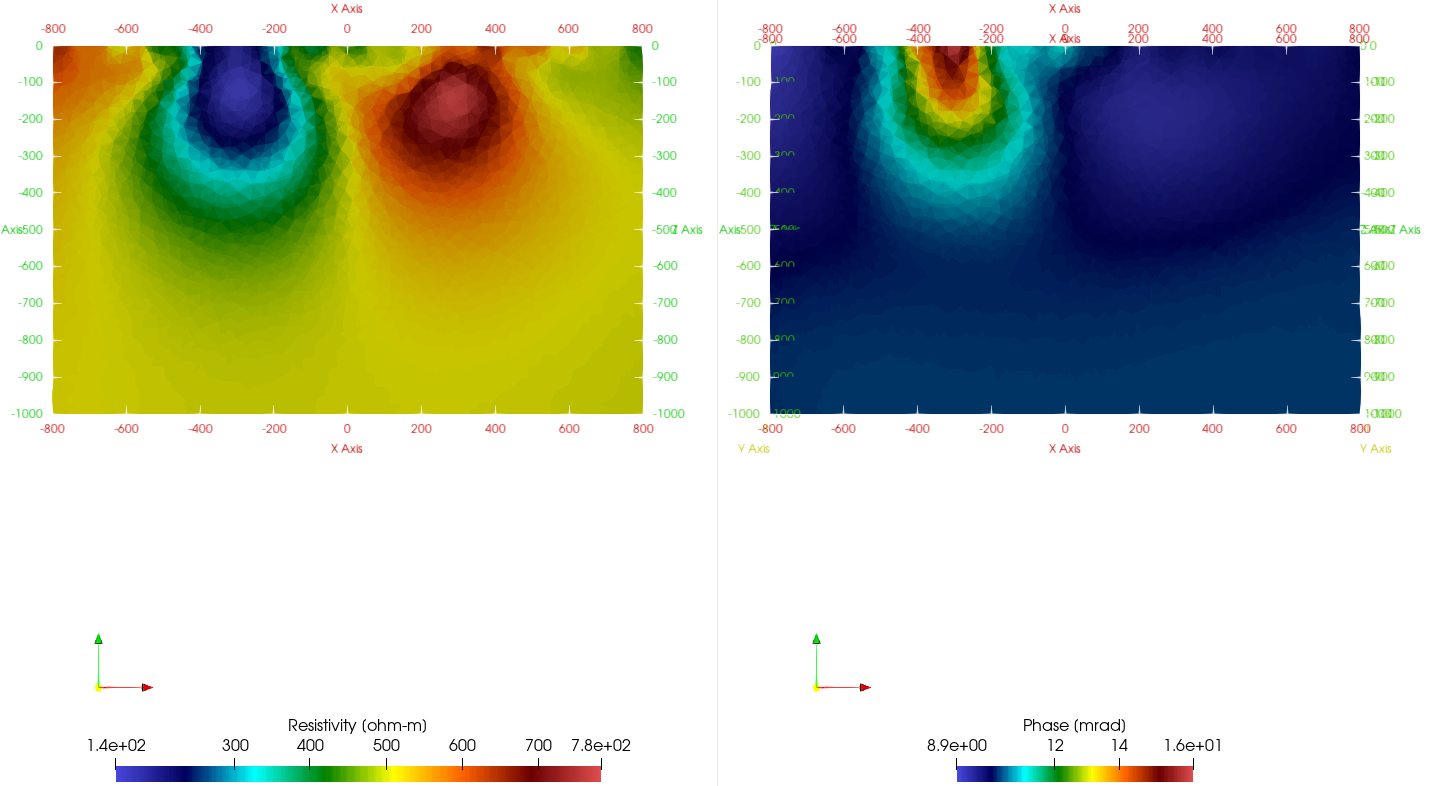
\includegraphics[width=7.0in]{figures/inversion_dcr_ip.png}}
\caption{Inversion model section view.}
\label{fig:inversion}
\end{figure}







\bibliographystyle{plain}
\bibliography{references}

\end{document}
